% ------------------------------------------------------------
% LaTeX Template für die DHBW zum Schnellstart!
% Original: https://github.wdf.sap.corp/vtgermany/LaTeX-Template-DHBW
% ------------------------------------------------------------
% ---- Präambel mit Angaben zum Dokument
% LTeX: enabled=false

\documentclass[
	fontsize=12pt,           % Leitlinien sprechen von Schriftgröße 12.
	paper=A4,
	twoside=false,
	listof=totoc,            % Tabellen- und Abbildungsverzeichnis ins Inhaltsverzeichnis
	bibliography=totoc,      % Literaturverzeichnis ins Inhaltsverzeichnis aufnehmen
	titlepage,               % Titlepage-Umgebung anstatt \maketitle
	headsepline,             % horizontale Linie unter Kolumnentitel
	abstract,              % Überschrift einschalten, Abstract muss in {abstract}-Umgebung stehen
]{scrreprt}                  % Verwendung von KOMA-Report
\usepackage[utf8]{inputenc}  % UTF8 Encoding einschalten
\usepackage[ngerman]{babel}  % Neue deutsche Rechtschreibung
% \usepackage[T1]{fontenc}     % Ausgabe von westeuropäischen Zeichen (auch Umlaute)
% \usepackage{fontspec}
\usepackage{microtype}       % Trennung von Wörtern wird besser umgesetzt
\usepackage{lmodern}         % Nicht-gerasterte Schriftarten (bei MikTeX erforderlich)
\usepackage{graphicx}        % Einbinden von Grafiken erlauben
\usepackage{rotating}        % Rotieren von Grafiken ermöglichen
\usepackage{adjustbox}
\usepackage{wrapfig}         % Grafiken fließend im Text
\usepackage{setspace}        % Zeilenabstand \singlespacing, \onehalfspaceing, \doublespacing
\usepackage[
	%showframe,                % Ränder anzeigen lassen
	left=2.7cm, right=2.5cm,
	top=2.5cm,  bottom=2.5cm,
	includeheadfoot,
	a4paper
]{geometry}                      % Seitenlayout einstellen
\usepackage{scrlayer-scrpage}    % Gestaltung von Fuß- und Kopfzeilen
\usepackage[printonlyused]{acronym}             % Abkürzungen, Abkürzungsverzeichnis
\usepackage{titletoc}            % Anpassungen am Inhaltsverzeichnis
\contentsmargin{0.75cm}          % Abstand im Inhaltsverzeichnis zw. Punkt und Seitenzahl
\usepackage[                     % Klickbare Links (enth. auch "nameref", "url" Package)
  hidelinks,                     % Blende die "URL Boxen" aus.
  breaklinks=true                % Breche zu lange URLs am Zeilenende um
]{hyperref}
\usepackage[hypcap=true]{caption}% Anker Anpassung für Referenzen
\urlstyle{same}                  % Aktuelle Schrift auch für URLs
% Anpassung von autoref für Gleichungen (ergänzt runde Klammern) und Algorithm.
% Anstatt "Listing" kann auch z.B. "Code-Ausschnitt" verwendet werden. Dies sollte
% jedoch synchron gehalten werden mit \lstlistingname (siehe weiter unten).
\addto\extrasngerman{%
	\def\equationautorefname~#1\null{Gleichung~(#1)\null}
	\def\lstnumberautorefname{Zeile}
	\def\lstlistingautorefname{Listing}
	\def\algorithmautorefname{Algorithmus}
	% Damit einheitlich "Abschnitt 1.2[.3]" verwendet wird und nicht "Unterabschnitt 1.2.3"
	% \def\subsectionautorefname{Abschnitt}
}

% ---- Abstand verkleinern von der Überschrift 
\renewcommand*{\chapterheadstartvskip}{\vspace*{.5\baselineskip}}

% Hierdurch werden Schusterjungen und Hurenkinder vermieden, d.h. einzelne Wörter
% auf der nächsten Seite oder in einer einzigen Zeile.
% LaTeX kann diese dennoch erzeugen, falls das Layout ansonsten nicht umsetzbar ist.
% Diese Werte sind aber gute Startwerte.
\widowpenalty10000
\clubpenalty10000

% ---- Für das Quellenverzeichnis
\usepackage[
	backend = biber,                % Verweis auf biber
	language = auto,
	style = numeric,                % Nummerierung der Quellen mit Zahlen
	sorting = none,                 % none = Sortierung nach der Erscheinung im Dokument
	sortcites = true,               % Sortiert die Quellen innerhalb eines cite-Befehls
	block = space,                  % Extra Leerzeichen zwischen Blocks
	hyperref = true,                % Links sind klickbar auch in der Quelle
	%backref = true,                % Referenz, auf den Text an die zitierte Stelle
	bibencoding = auto,
	giveninits = true,              % Vornamen werden abgekürzt
	doi=false,                      % DOI nicht anzeigen
	isbn=false,                     % ISBN nicht anzeigen
    alldates=short                  % Datum immer als DD.MM.YYYY anzeigen
]{biblatex}
\addbibresource{library.bib}
\setcounter{biburlnumpenalty}{3000}     % Umbruchgrenze für Zahlen
\setcounter{biburlucpenalty}{6000}      % Umbruchgrenze für Großbuchstaben
\setcounter{biburllcpenalty}{9000}      % Umbruchgrenze für Kleinbuchstaben
\DeclareNameAlias{default}{family-given}  % Nachname vor dem Vornamen
\AtBeginBibliography{\renewcommand{\multinamedelim}{\addslash\space
}\renewcommand{\finalnamedelim}{\multinamedelim}}  % Schrägstrich zwischen den Autorennamen
\DefineBibliographyStrings{german}{
  urlseen = {Einsichtnahme:},                      % Ändern des Titels von "besucht am"
}
\usepackage[babel,german=quotes]{csquotes}         % Deutsche Anführungszeichen + Zitate


% ---- Für Mathevorlage
\usepackage{amsmath}    % Erweiterung vom Mathe-Satz
\usepackage{amssymb}    % Lädt amsfonts und weitere Symbole
\usepackage{MnSymbol}   % Für Symbole, die in amssymb nicht enthalten sind.

% ---- Für chemische Formeln
\usepackage{mhchem}

% ---- Für Quellcodevorlage
\usepackage{scrhack}                    % Hack zur Verw. von listings in KOMA-Script
\usepackage{listings}                   % Darstellung von Quellcode
\usepackage{xcolor}                     % Einfache Verwendung von Farben
% -- Eigene Farben für den Quellcode
\definecolor{JavaLila}{rgb}{0.4,0.1,0.4}
\definecolor{JavaGruen}{rgb}{0.3,0.5,0.4}
\definecolor{JavaBlau}{rgb}{0.0,0.0,1.0}
\definecolor{ABAPKeywordsBlue}{HTML}{6000ff}
\definecolor{ABAPCommentGrey}{HTML}{808080}
\definecolor{ABAPStringGreen}{HTML}{4da619}
\definecolor{PyKeywordsBlue}{HTML}{0000AC}
\definecolor{PyCommentGrey}{HTML}{808080}
\definecolor{PyStringGreen}{HTML}{008080}
% -- Farben für ABAP CDS
\definecolor{CDSString}{HTML}{FF8C00}
\definecolor{CDSKeywords}{HTML}{6000ff}
\definecolor{CDSAnnotation}{HTML}{00BFFF}
\definecolor{CDSComment}{HTML}{808080}
\definecolor{CDSFunc}{HTML}{FF0000}

% -- Default Listing-Styles

\lstset{
	% Das Paket "listings" kann kein UTF-8. Deswegen werden hier 
	% die häufigsten Zeichen definiert (ä,ö,ü,...)
	literate=%
		{á}{{\'a}}1 {é}{{\'e}}1 {í}{{\'i}}1 {ó}{{\'o}}1 {ú}{{\'u}}1
		{Á}{{\'A}}1 {É}{{\'E}}1 {Í}{{\'I}}1 {Ó}{{\'O}}1 {Ú}{{\'U}}1
		{à}{{\`a}}1 {è}{{\`e}}1 {ì}{{\`i}}1 {ò}{{\`o}}1 {ù}{{\`u}}1
		{À}{{\`A}}1 {È}{{\'E}}1 {Ì}{{\`I}}1 {Ò}{{\`O}}1 {Ù}{{\`U}}1
		{ä}{{\"a}}1 {ë}{{\"e}}1 {ï}{{\"i}}1 {ö}{{\"o}}1 {ü}{{\"u}}1
		{Ä}{{\"A}}1 {Ë}{{\"E}}1 {Ï}{{\"I}}1 {Ö}{{\"O}}1 {Ü}{{\"U}}1
		{â}{{\^a}}1 {ê}{{\^e}}1 {î}{{\^i}}1 {ô}{{\^o}}1 {û}{{\^u}}1
		{Â}{{\^A}}1 {Ê}{{\^E}}1 {Î}{{\^I}}1 {Ô}{{\^O}}1 {Û}{{\^U}}1
		{œ}{{\oe}}1 {Œ}{{\OE}}1 {æ}{{\ae}}1 {Æ}{{\AE}}1 {ß}{{\ss}}1
		{ű}{{\H{u}}}1 {Ű}{{\H{U}}}1 {ő}{{\H{o}}}1 {Ő}{{\H{O}}}1
		{ç}{{\c c}}1 {Ç}{{\c C}}1 {ø}{{\o}}1 {å}{{\r a}}1 {Å}{{\r A}}1
		{€}{{\euro}}1 {£}{{\pounds}}1 {«}{{\guillemotleft}}1
		{»}{{\guillemotright}}1 {ñ}{{\~n}}1 {Ñ}{{\~N}}1 {¿}{{?`}}1,
	breaklines=true,        % Breche lange Zeilen um 
	breakatwhitespace=true, % Wenn möglich, bei Leerzeichen umbrechen
	% Symbol für Zeilenumbruch einfügen
	prebreak=\raisebox{0ex}[0ex][0ex]{\ensuremath{\rhookswarrow}},
	postbreak=\raisebox{0ex}[0ex][0ex]{\ensuremath{\rcurvearrowse\space}},
	tabsize=4,                                 % Setze die Breite eines Tabs
	basicstyle=\ttfamily\small,                % Grundsätzlicher Schriftstyle
	columns=fixed,                             % Besseres Schriftbild
	numbers=left,                              % Nummerierung der Zeilen
	%frame=single,                             % Umrandung des Codes
	showstringspaces=false,                    % Keine Leerzeichen hervorheben
	keywordstyle=\color{blue},
	ndkeywordstyle=\bfseries\color{darkgray},
	identifierstyle=\color{black},
	commentstyle=\itshape\color{JavaGruen},   % Kommentare in eigener Farbe
	stringstyle=\color{JavaBlau},             % Strings in eigener Farbe,
	captionpos=b,                             % Bild*unter*schrift
	xleftmargin=5.0ex
}

% ---- Eigener JAVA-Style für den Quellcode
\renewcommand{\ttdefault}{pcr}               % Schriftart, welche auch fett beinhaltet
\lstdefinestyle{EigenerJavaStyle}{
	language=Java,                             % Syntax Highlighting für Java
	%frame=single,                             % Umrandung des Codes
	keywordstyle=\bfseries\color{JavaLila},    % Keywords in eigener Farbe und fett
	commentstyle=\itshape\color{JavaGruen},    % Kommentare in eigener Farbe und italic
	stringstyle=\color{JavaBlau}               % Strings in eigener Farbe
}

% ---- Eigener ABAP-Style für den Quellcode
\renewcommand{\ttdefault}{pcr}
\lstdefinestyle{EigenerABAPStyle}{
	language=[R/3 6.10]ABAP,
	morestring=[b]\|,                          % Für Pipe-Strings
	morestring=[b]\`,                          % für Backtick-Strings
	keywordstyle=\bfseries\color{ABAPKeywordsBlue},
	commentstyle=\itshape\color{ABAPCommentGrey},
	stringstyle=\color{ABAPStringGreen},
	tabsize=2,
	morekeywords={
		types,
		@data,
		as,
		lower,
		start,
		selection,
		order,
		by,
		inner,
		join,
		key,
		end,
		cast
	}
}

% ---- Eigener Python-Style für den Quellcode
\renewcommand{\ttdefault}{pcr}
\lstdefinestyle{EigenerPythonStyle}{
	language=Python,
	columns=flexible,
	keywordstyle=\bfseries\color{PyKeywordsBlue},
	commentstyle=\itshape\color{PyCommentGrey},
	stringstyle=\color{PyStringGreen}
}

%----- ABAP-CDS-View language
\lstdefinelanguage{ABAPCDS}{
	sensitive=false,
	%Keywords
	morekeywords={define,
		view,
		as,
		select,
		from,
		inner,
		join,
		on,
		key,
		case,
		when,
		then,
		else,
		end,
		true,
		false,
		cast,
		where,
		and,
		distinct,
		group,
		by,
		having,
		min,
		sum,
		max,
		count,
		avg
	},
	%Methoden
	morekeywords=[2]{
		div,
		currency\_conversion,
		dats\_days\_between,
		concat\_with\_space,
		dats\_add_days,
		dats\_is\_valid,
		dats\_add\_months,
		unit\_conversion,
		division,
		mod,
		abs,
		floor,
		ceil,
		round,
		concat,
		replace,
		substring,
		left,
		right,
		length
	},
	morecomment=[s][\color{CDSAnnotation}]{@}{:},
	morecomment=[l][\itshape\color{CDSComment}]{//},
	morecomment=[s][\itshape\color{CDSComment}]{/*}{*/},
	morestring=[b][\color{CDSString}]',
	keywordstyle=\bfseries\color{CDSKeywords},
	keywordstyle=[2]\color{CDSFunc}
}

  % Weitere Details sind ausgelagert

\usepackage{algorithm}                  % Für Algorithmen-Umgebung (ähnlich wie lstlistings Umgebung)
\usepackage{algpseudocode}              % Für Pseudocode. Füge "[noend]" hinzu, wenn du kein "endif",
                                        % etc. haben willst.

\makeatletter                           % Sorgt dafür, dass man @ in Namen verwenden kann.
                                        % Ansonsten gibt es in der nächsten Zeile einen Compilefehler.
\renewcommand{\ALG@name}{Algorithmus}   % Umbenennen von "Algorithm" im Header der Listings.
\makeatother                            % Zeichen wieder zurücksetzen
\renewcommand{\lstlistingname}{Listing} % Erlaubt das Umbenennen von "Listing" in anderen Titel.

% ---- Tabellen
\usepackage{booktabs}  % Für schönere Tabellen. Enthält neue Befehle wie \midrule
\usepackage{multirow}  % Mehrzeilige Tabellen
\usepackage{siunitx}   % Für SI Einheiten und das Ausrichten Nachkommastellen
\sisetup{locale=DE, range-phrase={~bis~}, output-decimal-marker={,}} % Damit ein Komma und kein Punkt verwendet wird.
\usepackage{xfrac} % Für siunitx Option "fraction-function=\sfrac"

% ---- Für Definitionsboxen in der Einleitung
\usepackage{amsthm}                     % Liefert die Grundlagen für Theoreme
\usepackage[framemethod=tikz]{mdframed} % Boxen für die Umrandung
% ---- Definition für Highlight Boxen

% ---- Grundsätzliche Definition zum Style
\newtheoremstyle{defi}
  {\topsep}         % Abstand oben
  {\topsep}         % Abstand unten
  {\normalfont}     % Schrift des Bodys
  {0pt}             % Einschub der ersten Zeile
  {\bfseries}       % Darstellung von der Schrift in der Überschrift
  {:}               % Trennzeichen zwischen Überschrift und Body
  {.5em}            % Abstand nach dem Trennzeichen zum Body Text
  {\thmname{#3}}    % Name in eckigen Klammern
\theoremstyle{defi}

% ------ Definition zum Strich vor eines Texts
\newmdtheoremenv[
  hidealllines = true,       % Rahmen komplett ausblenden
  leftline = true,           % Linie links einschalten
  innertopmargin = 0pt,      % Abstand oben
  innerbottommargin = 4pt,   % Abstand unten
  innerrightmargin = 0pt,    % Abstand rechts
  linewidth = 3pt,           % Linienbreite
  linecolor = gray!40,       % Linienfarbe
]{defStrich}{Definition}     % Name der des formats "defStrich"

% ------ Definition zum Eck-Kasten um einen Text
\newmdtheoremenv[
  hidealllines = true,
  innertopmargin = 6pt,
  linecolor = gray!40,
  singleextra={              % Eck-Markierungen für die Definition
    \draw[line width=3pt,gray!50,line cap=rect] (O|-P) -- +(1cm,0pt);
    \draw[line width=3pt,gray!50,line cap=rect] (O|-P) -- +(0pt,-1cm);
    \draw[line width=3pt,gray!50,line cap=rect] (O-|P) -- +(-1cm,0pt);
    \draw[line width=3pt,gray!50,line cap=rect] (O-|P) -- +(0pt,1cm);
  }
]{defEckKasten}{Definition}  % Name der des formats "defEckKasten"  % Weitere Details sind ausgelagert

% ---- Für Todo Notes
\usepackage{todonotes}
\setlength {\marginparwidth }{2cm}      % Abstand für Todo Notizen

\lstdefinelanguage{JavaScript}{
  morekeywords=[1]{break, case, catch, continue, debugger, default, delete, do, else, finally, for, function, if, in, instanceof, new, return, switch, this, throw, try, typeof, var, void, while, with, require, then, const},
  morecomment=[l]{//},
  morecomment=[s]{/*}{*/},
  morestring=[b]{'},
  morestring=[b]{"},
  morestring=[b]{`},
%   alsoletter={\\'},
  stringstyle=\color[rgb]{0.3,0.5,0.4},
  sensitive=true
}

\lstdefinelanguage{Docker}{
	% Keywords as defined in the language grammar
	morekeywords=[1]{%
	  FROM,RUN,COPY,WORKDIR,LABEL,USER,ENTRYPOINT,EXPOSE,CMD},
	% Built-in functions
	morekeywords=[2]{},
	% Pre-declared types
	morekeywords=[3]{},
	% Constants and zero value
	morekeywords=[4]{},
	% Strings : "foo", 'bar', `baz`
	morestring=[b]{"},
	morestring=[b]{'},
	morestring=[b]{`},
	% Comments : /* cpmment */ and // comment
	comment=[l]{\#},
	morecomment=[s]{/*}{*/},
	stringstyle=\color[rgb]{0.3,0.5,0.4},
	% Options
	sensitive=true
}

\usepackage{xurl}
\usepackage{tikz}

% ---- Elektronische Version oder Gedruckte Version?
% ---- Unterschied: Die elektronische Version enthält keinen Platzhalter für die Unterschrift
\usepackage{ifthen}
\newboolean{e-Abgabe}
\setboolean{e-Abgabe}{false}    % false=gedruckte Fassung

% ---- Persönlichen Daten:
\newcommand{\titel}{Erlernen von Hindernisumfahrung mithilfe von Reinforcement Learning}
\newcommand{\titelheader}{RL-Hindernisumfahrung}
\newcommand{\arbeit}{Studienarbeit (T3\_3101)}
\newcommand{\studiengang}{Informatik}
\newcommand{\studienjahr}{2020}
\newcommand{\autor}{Yannik Schiebelhut}
\newcommand{\autorReverse}{Schiebelhut, Yannik}
\newcommand{\verfassungsort}{Karlsruhe}
\newcommand{\matrikelnr}{3354235}
\newcommand{\kurs}{TINF20B1}
\newcommand{\bearbeitungsmonat}{Mai 2023}
\newcommand{\abgabe}{22. Mai 2023}
\newcommand{\bearbeitungszeitraum}{14.10.2022 - 22.05.2023}
\newcommand{\firmaName}{SAP SE}
\newcommand{\firmaStrasse}{Dietmar-Hopp-Allee 16}
\newcommand{\firmaPlz}{69190 Walldorf, Deutschland}
\newcommand{\betreuerFirma}{Alexander Schaefer}
\newcommand{\betreuerDhbw}{Florian Stöckl}

% ---- Metainformation für das PDF Dokument
\hypersetup{
	pdftitle    = {\titel},
	pdfsubject  = {\arbeit},
	pdfauthor   = {\autor},
	%pdfkeywords = {Keywords angeben},
	pdfcreator  = {LaTeX},
	%pdfproducer = {in der Regel pdfTeX}
}

% ---- Definition der Kopf- und Fußzeilen
\clearscrheadfoot                               % Löschen von LaTeX Standard
\automark[section]{chapter}                     % Füllen von section und chapter
\renewcommand*{\chaptermarkformat}{}            % Entfernt die Kapitelnummer
\renewcommand*{\sectionmarkformat}{}            % Entfernt die Sectionnummer
% Angaben [für "plain"]{für "scrheadings"}
% \ihead[]{\titelheader}                          % Kopfzeile links
\ihead{\ifthenelse{\value{chapter}>0}{\chaptername~\thechapter}{}}
\chead[]{}                                      % Kopfzeile mitte
% \ohead[]{\rightmark}                            % Kopfzeile rechts
\ohead{\ifthenelse{\value{chapter}>0}{\headmark}{}}
\ifoot[]{}                                      % Fußzeile links
\cfoot*{\sffamily\pagemark}                     % Fußzeile mitte
\ofoot[]{}                                      % Fußzeile rechts
\KOMAoptions{
   headsepline = 0.2pt,                         % Liniendicke Kopfzeile
   footsepline = false                          % Liniendicke Fußzeile
}

% ---- Hilfreiches
\newcommand{\zB}{z.\,B. }   % "z.B." mit kleinem Leeraum dazwischen (ohne wäre nicht korrekt)
\newcommand{\dash}{d.\,h. }
\newcommand{\Dash}{D.\,h. }

\newcommand{\code}[1]{\texttt{#1}} % Ist einfacher zu schreiben als ständig \texttt und erlaubt
                                   % Änderungen im Nachhinein, wenn man z.B. Inline-Code anders stylen möchte.

% ---- Silbentrennung (falls LaTeX defaults falsch / nicht gewünscht sind)
\hyphenation{HANA}         % anstatt HA-NA
\hyphenation{Graph-Script} % anstatt GraphS-cript

% ---- Beginn des Dokuments
\begin{document}
\setlength{\parindent}{0pt}              % Keine Paragraphen Einrückung.
                                         % Dafür haben wir den Abstand zwischen den Paragraphen.
\setcounter{secnumdepth}{2}              % Nummerierungstiefe fürs Inhaltsverzeichnis
\setcounter{tocdepth}{1}                 % Tiefe des Inhaltsverzeichnisses. Ggf. so anpassen,
                                         % dass das Verzeichnis auf eine Seite passt.
\sffamily                                % Serifenlose Schrift verwenden.

% ---- Vorspann
% ------ Titelseite
\singlespacing
\thispagestyle{empty}
\begin{titlepage}
\enlargethispage{4cm}

\begin{figure}
	
\includegraphics[height=2.5cm]{Bilder/Logos/Logo_DHBW.pdf}
	\centering
\end{figure} 
\vspace*{0.1cm}

\begin{center}
	\huge{\textbf{\titel}}\\[1.5cm]
	\Large{\textbf{\arbeit}}\\[0.5cm]
	\normalsize{im Rahmen der Prüfung zum\\[1ex] \textbf{Bachelor of Science (B.Sc.)}}\\[0.5cm]
	\Large{des Studienganges \studiengang}\\[1ex]
	\normalsize{an der Dualen Hochschule Baden-Württemberg Karlsruhe}\\[1cm]
	\normalsize{von}\\[1ex] \Large{\textbf{\autor}} \\[1cm]
\end{center}

\begin{center}
	\vfill
	\begin{tabular}{ll}
		Abgabedatum:                     & \abgabe \\[0.2cm]
		Bearbeitungszeitraum:            & \bearbeitungszeitraum \\[0.2cm]
		Matrikelnummer, Kurs:            & \matrikelnr , \kurs \\[0.2cm]
		% Ausbildungsfirma:                & \firmaName \\
		%                                  & \firmaStrasse \\
		%                                  & \firmaPlz \\[0.2cm]
		% Betreuer der Ausbildungsfirma:   & \betreuerFirma \\[0.2cm]
		Gutachter der Dualen Hochschule: & \betreuerDhbw \\[2cm]
	\end{tabular} 
\end{center}
\end{titlepage}
  % Titelseite
\newcounter{savepage}
\pagenumbering{Roman}                    % Römische Seitenzahlen
\onehalfspacing

% ------ Erklärung, Sperrvermerk, Abstact
\chapter*{Eidesstattliche Erklärung}
Ich versichere hiermit, dass ich meine \arbeit{} mit dem Thema:
\begin{quote}
	\textit{\titel}
\end{quote} 
gemäß § 5 der \enquote{Studien- und Prüfungsordnung DHBW Technik} vom 29. September 2017 selbstständig verfasst und keine anderen als die angegebenen Quellen und Hilfsmittel benutzt habe. Die Arbeit wurde bisher keiner anderen Prüfungsbehörde vorgelegt und auch nicht veröffentlicht.

\vspace{0.25cm}

Ich versichere zudem, dass die eingereichte elektronische Fassung mit der gedruckten Fassung übereinstimmt.

\vspace{1cm}

\verfassungsort, den \today \\[0.5cm]
\ifthenelse{\boolean{e-Abgabe}}
	{\underline{Gez. \autor}}
	{\makebox[6cm]{\hrulefill}}\\ 
\autorReverse

\renewcommand{\abstractname}{Abstract} % Veränderter Name für das Abstract
\begin{abstract}
\begin{addmargin}[1.5cm]{1.5cm}        % Erhöhte Ränder, für Abstract Look
\thispagestyle{plain}                  % Seitenzahl auf der Abstract Seite

\begin{center}
\small\textit{- Deutsch -}             % Angabe der Sprache für das Abstract
\end{center}

\vspace{0.25cm}

Platzhalter


\end{addmargin}
\end{abstract}
\renewcommand{\abstractname}{Abstract} % Veränderter Name für das Abstract
\begin{abstract}
\begin{addmargin}[1.5cm]{1.5cm}        % Erhöhte Ränder, für Abstract Look
\thispagestyle{plain}                  % Seitenzahl auf der Abstract Seite

\begin{center}
\small\textit{- English -}             % Angabe der Sprache für das Abstract
\end{center}

\vspace{0.25cm}

% LTeX: language=en-US

Placeholder

\end{addmargin}
\end{abstract}

% ------ Inhaltsverzeichnis
\singlespacing
\tableofcontents

% ------ Verzeichnisse
\renewcommand*{\chapterpagestyle}{plain}
\pagestyle{plain}
% \chapter*{Formelverzeichnis}
\addcontentsline{toc}{chapter}{Formelverzeichnis} % Hinzufügen zum Inhaltsverzeichnis 

% Definition des neuen Befehls für das Einfügen der Abkürzung der Einheit
\newcommand{\acrounit}[1]{
  \acroextra{\makebox[18mm][l]{\si[per-mode=fraction,fraction-function=\sfrac]{#1}}}
}
\begin{acronym}[dmin] % längstes Kürzel wird verw. für den Abstand zw. Kürzel u. Text

	% Alphabetisch selbst sortieren - nicht verwendete Formeln rausnehmen!
	% Allgemein: \acro{KÜRZEL}[ABKÜRZUNG]{\acrounit{SI-EINHEIT}BESCHREIBUNG}

	\acro{A}[\ensuremath{A}]{\acrounit{mm^2}Fläche}	
	\acro{D}[\ensuremath{D}]{\acrounit{mm}Werkstückdurchmesser}	
	\acro{dmin}[\ensuremath{d\textsubscript{min}}]{\acrounit{mm}kleinster Schaftdurchmesser}	
	\acro{L1}[\ensuremath{L\textsubscript{1}}]{\acrounit{mm}Länge des Werkstückes Nr. 1}	
	\acro{Fwinkel}[]{\acrounit{Grad}Freiwinkel}	
	\acro{Kwinkel}[]{\acrounit{Grad}Keilwinkel}

\end{acronym}

\chapter*{Abkürzungsverzeichnis}
\addcontentsline{toc}{chapter}{Abkürzungsverzeichnis} % Hinzufügen zum Inhaltsverzeichnis 

\begin{acronym}[PPO] % längstes Kürzel wird verw. für den Abstand zw. Kürzel u. Text

	% Alphabetisch selbst sortieren - nicht verwendete Kürzel rausnehmen!
	% \acro{AIR}{Adobe Integrated Runtime}
	% \acro{AJAX}{Asynchronous Javascript and XML}
	% \acro{ANSI}{American National Standards Institute}
	% \acro{api}[API]{Application Programming Interface}
	% \acro{AR}{Augmented Reality}
	% \acro{BAPI}{Business Application Programming Interface}
	% \acro{BIOS}{Basic Input Output System}
	% \acro{bpmn}[BPMN]{Business Process Model and Notation}
	% \acro{ccwf}[ccWF]{Cross-Company Workflow}
	% \acro{CDMA}{Code Division Multiple Access}
	% \acro{csv}[CSV]{Comma-Separated Values}
	% \acro{erp}[ERP]{Enterprise Resource Planning}
	% \acro{hs2}[HS2]{High Speed 2}
	% \acro{HTTP}{Hypertext Transfer Protocol}
	% \acro{HTTPS}{Hypertext Transfer Protocol Secure}
	% \acro{IP}{Internet Protocol}
	% \acro{ISBN}{Internationale Standardbuchnummer}
	% \acrodefplural{ISBN}[ISBNs]{Internationale Standardbuchnummern}
	% \acro{JSON}{JavaScript Object Notation}
	% \acro{kpi}[KPI]{Key Performance Indicator}
	\acro{mdp}[MDP]{Markov Decision Process}
	% \acro{OData}{Open Data Protocol}
	\acro{ppo}[PPO]{Proximal Policy Optimization}
	% \acro{SDK}{Software Development Kit}
	% \acro{SEO}{Search Engine Optimization}
	% \acro{sql}[SQL]{Structured Query Language}
	% \acro{SSH}{Secure Shell}
	% \acro{UEFI}{Unified Extensible Firmware Interface}
	% \acro{URI}{Uniform Resource Identifier}
	% \acro{USB}{Universal Serial Bus}
	% \acro{VLAN}{Virtual Local Area Network}
	% \acro{WYSISWG}{What You See Is What You Get}
	% \acro{xes}[XES]{eXtensible Event Stream}
	% \acro{XSL}{Extensible Stylesheet Language}

\end{acronym}
\listoffigures                          % Erzeugen des Abbildungsverzeichnisses 
% \listoftables                           % Erzeugen des Tabellenverzeichnisses
\renewcommand{\lstlistlistingname}{Quellcodeverzeichnis}
\lstlistoflistings                      % Erzeugen des Listenverzeichnisses
\setcounter{savepage}{\value{page}}


% ---- Inhalt der Arbeit
\cleardoublepage
\pagenumbering{arabic}                  % Arabische Seitenzahlen für den Hauptteil
\setlength{\parskip}{0.5\baselineskip}  % Abstand zwischen Absätzen
\rmfamily
\renewcommand*{\chapterpagestyle}{scrheadings}
\pagestyle{scrheadings}
\onehalfspacing
% \include{content goes here}
\chapter{Einleitung}
\label{sec:einleitung}
Die Robotik ist ein breites Forschungsfeld mit praktisch grenzenlosen Möglichkeiten.
Die Fähigkeit, sich zu bewegen, ist dabei besonders spannend, da sie die Flexibilität der Einsatzmöglichkeiten für Roboter stark erhöht.
Roboter mit Beinen stellen sich besonders heraus.
Mit Inspirationen aus Mensch- und Tierreich bieten diese das Potenzial, sich in jedem denkbaren Terrain fortzubewegen, das auch für Menschen zugänglich ist oder sogar in Gebiete vorzudringen, die uns verwehrt bleiben.
Im Vergleich zu anderen Fortbewegungsarten stellt die stabile Koordination von mehreren Beinen, die jeweils aus mehreren Gelenken bestehen, allerdings eine große Herausforderung für die technische Umsetzung dar.
In der Regel sind für die Programmierung solcher Roboter eine sehr genaue Kenntnis der Maschine und deren Dynamik vonnöten.

In den vergangenen Jahren wird deshalb verstärkt erforscht, wie Roboter sich diese Fähigkeiten selbstständig mittels Reinforcement Learning beibringen können.
In einer vorangegangenen Studienarbeit wurden am Beispiel eines eigens dafür gebauten, spinnenartigen, vierbeinigen Roboters Möglichkeiten erforscht, um diesen mittels selbst gelernter Bewegungsabläufe möglichst effizient und schnell geradlinig nach vorne zu bewegen.
Um den Trainingsprozess zu beschleunigen wurde dabei der Roboter in der Simulationsumgebung \enquote{Unity} nachgebaut und trainiert.

Für das Erfüllen eines praktischen Nutzens ist es jedoch in der Regel nicht ausreichend, wenn sich ein Roboter nur in eine feste Richtung bewegen kann.
Im Rahmen dieser Arbeit wird deshalb untersucht, wie dem Roboter beigebracht werden kann, einem gezielt übergebenen Pfad zu folgen.
Weiterhin soll der Roboter dabei Hindernisse, die sich auf diesem Pfad befinden, automatisch umsteuern und anschließend wieder auf den vorgebenen Pfad zurückkehren. % ggf Absatz hier
Dazu werden zunächst die Arbeitsumgebung und Ergebnisse der vorherigen Arbeit rekonstruiert.
Anschließend wird diskutiert, welche Änderungen am Roboter und dessen Simulationsumgebung vorgenommen werden müssen, um die erweiterten Anforderungen grundsätzlich erfüllen zu können.
Außerdem wird erläutert, wie die Aufgabe in sinnvolle Teilaufgaben gegliedert werden kann.
Zur Bearbeitung dieser Teilaufgaben wird dann ein Konzept erarbeitet, welches im Anschluss in der Simulationsumgebung, unter Zuhilfenahme des ML-Agents-Toolkits, mittels des \acl{ppo}-Algorithmus ein Proof-of-Concept trainiert.
Anhand der Ergebnisse dieses Trainingsprozesses wird evaluiert, ob das entwickelte Konzept einen erfolgversprechenden Lösungsansatz darstellt und welche Verbesserungen vorgenommen werden sollten.

% \begin{itemize}
%     \item Roboter sind ein breites Forschungsfeld mit grenzenlosen Möglichkeiten
%     \item Fähigkeit, sich zu bewegen ist besonders spannend für die Robotik, da es die Einsatzmöglichkeiten für Roboter stark erweitert
%     \item dabei insbesondere mehrbeinige Roboter interessant
%     \item mit Inspiration aus Menschen- und Tierreich sind diese fähig, sich in praktisch jedem denkbaren Terrain fortzubewegen
%     \item im Vergleich zu anderen Fortbewegungsarten stellt stabile Koordination von Beinen jedoch eine große Herausforderung für die technische Umsetzung voraus
%     \item in der Regel sehr genaue Kenntnis des Roboters und dessen Dynamik vonnöten
    
%     \item in den vergangenen Jahren wird deshalb verstärkt erforscht, wie Roboter sich diese Fähigkeit gegebenenfalls selbstständig mittels Reinforcement Learning beibringen können
%     \item in einer vorangegangenen Studienarbeit wurden am Beispiel eines eigens dafür gebauten, vierbeinigen Roboters Möglichkeiten erforscht, um diesen möglichst effizient und schnell geradlinig nach vorne zu bewegen
%     \item dabei wurde der Roboter in der Simulationsumgebung \enquote{Unity} trainiert
%     \item für das Erfüllen eines praktischen Nutzens ist es jedoch in der Regel nicht ausreichend, wenn sich ein Roboter nur in eine Richtung bewegen kann
%     \item im Rahmen dieser Arbeit wird deshalb untersucht, wie dem Roboter beigebracht werden kann, einem gezielt übergebenen Pfad zu folgen
%     \item weiterhin soll der Roboter Hindernisse, die sich auf diesem Pfad befinden, automatisch umsteuern und anschließend wieder auf den vorgegebenen Pfad zurückkehren
    
%     \item dazu werden zunächst die Ergebnisse und Arbeitsumgebung der vorherigen Arbeit rekonstruiert
%     \item anschließend wird diskutiert, welche Änderungen am Roboter und dessen Simulationsumgebung vorgenommen werden müssen, um die erweiterten Anforderungen grundsätzlich erfüllen zu können
%     \item außerdem wird erläutert, wie die Aufgabe in sinnvolle Teilaufgaben gegliedert werden kann
%     \item zur Bearbeitung dieser Teilaufgaben wird dann ein Konzept erarbeitet, welches im Anschluss in der Simulationsumgebung unter Zuhilfenahme des ML-Agents-Toolkits als Proof-of-Concept trainiert wird
%     \item Proximal-Policy-Optimization
% \end{itemize}

\chapter{Grundlagen}
Wie in \autoref{sec:einleitung} bereits angedeutet, werden in dieser Arbeit Methoden aus dem Bereich der künstlichen Intelligenz verwendet, um das gestellte Problem zu lösen.
Nachfolgend werden die wichtigsten Grundlagen zum Verständnis der Ausarbeitungen erläutert.
Weiterhin wird kurz auf die zur Simulation verwendete Software eingegangen.
Im Rahmen der konzeptuellen Planung wird auch von mathematischen Grundlagen des dreidimensionalen Raums Gebrauch gemacht, welche deshalb ebenfalls kurz beleuchtet werden.
Im Anschluss wird die Projektbasis vorgestellt, auf der diese Arbeit aufbaut.

\section{Machine Learning}
Machine Learning ist eine Unterkategorie der künstlichen Intelligenz und bezeichnet einen automatisierten Prozess, der es Computern ermöglicht, eigenständig aus Trainingsdaten zu lernen und sich mit der Zeit zu verbessern, ohne explizit zur Lösung einer Aufgabe programmiert zu werden.
Machine Learning Algorithmen können Muster in Daten entdecken und aus ihnen lernen, um eigene Prognosen und Entscheidungen zu treffen.

In der Regel wird Machine Learning in folgende Teilbereiche untergliedert \cite{monkeylearnIntroductionMachine}:
\begin{itemize}
    \item \textbf{Supervised Learning:}
    Ein Modell wird anhand von gelabelten Trainingsdaten trainiert.
    Ein Datentupel besteht dabei aus einer Eingabe und der dazu gewollten Ausgabe.
    Der Algorithmus sucht beim Training nach Zusammenhängen und Abhängigkeiten um anschließend, die gelernten Daten generalisierend, Ausgaben für unbekannte Eingaben generieren zu können.
    Üblicherweise wird Supervised Learning für Regressions- und Klassifikationsprobleme eingesetzt.

    \item \textbf{Unsupervised Learning:}
    Wird in der Regel für Clusterbildung von unbeschrifteten Trainingsdaten verwendet.
    Der Algorithmus muss dabei selbstständig nach Mustern in den Daten suchen.
    Unsupervised Learning kann dabei helfen, Einblicke in große Datensätzen zu erhalten, um etwa versteckte Trends zu entdecken.

    \item \textbf{Semi-Supervised Learning:}
    Für das Training werden beim Semi-Supervised Learning sowohl ein kleiner gelabelter, als auch ein großer ungelabelter Datensatz verwendet.
    Dabei werden die Vorzüge von Supervised und Unsupervised Learning miteinander verbunden.
    Interessant ist dies vor allem bei sehr großen Datensätzen (zum Beispiel bei Bild-Klassifizierung), da die Labelung der Daten in der Regel manuell erfolgen muss.

    \item \textbf{Reinforcement Learning:}
    Beim Reinforcement Learning kann ein Agent Aktionen tätigen, für die er entweder belohnt oder bestraft wird.
    Es ist sein Ziel, selbstständig ein bestmögliches Verhalten zu lernen, um seine Belohnung zu maximieren.
    Dabei werden keine Trainingsdaten verwendet.
    Der Agent lernt ausschließlich aus seinen eigenen Erfahrungen und Fehlern.
    Reinforcement Learning findet vor allem in den Bereichen Robotik und Videospiele Einsatz und wird in dieser Arbeit verwendet.
\end{itemize}

% \begin{itemize}
%     \item Unterkategorie der künstlichen Intelligenz
%     \item ML ist ein automatisierter Prozess, der ...
%     \item ermöglicht Computern, eigenständig aus Trainingsdaten zu lernen und sich mit der Zeit zu verbessern, ohne explizit programmiert zu werden
%     \item ML Algorithmen können Muster in Daten entdecken und aus ihnen lernen, um eigene Voraussagen und Entscheidungen zu treffen
    
%     \item verschiedene Teilbereiche
%     \item Supervised Learning
    
%     Vorhersagen von gelabelten Trainingsdaten
%     Datensatz: Input mit gewolltem Output
%     \item Unsupervised Learning
    
%     Einblicke und Beziehungen in unbeschrifteten Daten
%     Modelle müssen selbstständig Muster finden
%     Clustering
%     kann helfen, versteckte Muster oder Trends zu entdecken
%     \item Semi-Supervised Learning
    
%     kleiner Teil gelabelter Daten, viele ungelabelte
%     besonders für große Datensätze interessant, Bild-Klassifizierung
%     \item Reinforcement Learning
    
%     vor allem im Bereich Robotik und Videospiele vertreten
%     Agent kann Aktionen tätigen, für die er belohnt oder bestraft wird
%     es ist sein Ziel, ein bestmögliches Verhalten zu lernen, um seine Belohnung zu maximieren
%     keine Trainingsdaten, Lernen aus eigenen Fehlern
%     in diesem Kontext besonders interessant wird verwendet

%     \item \cite{monkeylearnIntroductionMachine}
% \end{itemize}

\subsection{Reinforcement Learning}
Reinforcement Learning ist ein rechnerischer Ansatz, um zielorientierte Lern- und Entscheidungsprozesse zu verstehen und nachzubilden.
Wie oben beschrieben, steht dabei ein \emph{Agent} im Zentrum, der aus der direkten Interaktion mit seiner \emph{Umgebung (engl. Environment)} lernt, ohne dabei eine beispielhafte Anleitung oder vollständige Modelle der Umgebung zu benötigen.
Das formale Framework des \emph{\acf{mdp}} wird genutzt, um die Interaktion zwischen dem lernenden Agent und seiner Umgebung zu definieren.
\acp{mdp} sind eine mathematisch idealisierte Form eines Reinforcement Learning Problems, für die präzise, theoretische Aussagen getroffen werden können \cite[13]{sutton2018rlintro}.
\autoref{fig:mdp} stellt die grundlegende Struktur eines Reinforcement Learning Problems dar.
Die einzelnen Bestandteile der Abbildung werden nachfolgend erläutert.

\begin{figure}
    \centering
    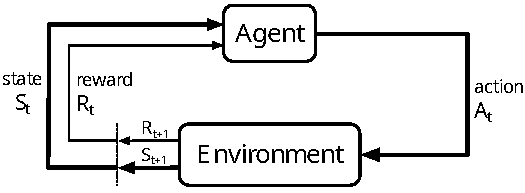
\includegraphics[width = 0.7\textwidth]{Bilder/MDP.pdf}
    \caption{Die Interaktion von Agent und Umgebung als \ac{mdp} \cite[48]{sutton2018rlintro}}
    \label{fig:mdp}
\end{figure}

Agents haben explizite Ziele, können Aspekte ihrer Umgebung wahrnehmen und \emph{Aktionen} $A$ auswählen, um mit ihrer Umgebung zu interagieren und diese zu beeinflussen.
Es wird davon ausgegangen, dass Reinforcement Learning diejenige Strategie des Machine Learning ist, die dem natürlichen Lernen von Menschen und Tieren am nächsten kommt.
Viele zentrale Algorithmen des Reinforcement Learnings sind ursprünglich durch biologische Systeme inspiriert \cite[4]{sutton2018rlintro}.

Besonders wichtig für Reinforcement Learning ist das Konzept von \emph{Zuständen} $S$.
Ein Zustand kann dabei als eine Art Signal verstanden werden, das dem Agent Informationen über den Zustand der Umgebung liefert.
Weiterhin definieren folgende Elemente ein Reinforcement Learning Problem:
\begin{itemize}
    \item \textbf{Policy} $\mathbf{\pi}$\textbf{:}
    Die Policy definiert, wie sich der Agent zu einer gegebenen Zeit verhält.
    Sie stellt ein Mapping zwischen den wahrgenommenen Zuständen der Umgebung und den durchzuführenden Aktionen dar.
    Die Policy ist hinreichend, um das Verhalten des Agents zu bestimmen \cite[6]{sutton2018rlintro}.

    \item \textbf{Reward-Signal} $\mathbf{R}$\textbf{:}
    Das Reward-Signal definiert das Ziel eines Reinforcement Learning Problems.
    Bei jedem \emph{Zeitschritt} $t$ sendet die Umgebung ein Skalar an den Agent.
    Das einzige Ziel des Agents ist die Maximierung des kumulativen Rewards.
    Der Reward ist die primäre Basis für Änderungen an der Policy \cite[6]{sutton2018rlintro}.

    \item \textbf{Value-Funktion} $\mathbf{V}$\textbf{:}
    Die Value-Funktion legt fest, welches Verhalten auf lange Sicht gut ist.
    Der Value eines Zustands ist der kumulierte Reward, den ein Agent, ausgehend von diesem Zustand, in der Zukunft erwarten kann.
    Values geben die langfristige Attraktivität von Zuständen an.
    Die Wahl einer Aktion wird auf Basis der Value-Einschätzung des aktuellen Zustands getroffen.
    Im Vergleich zum Reward-Signal sind Values allerdings deutlich schwerer zu bestimmen, da diese anhand einer Sequenz von Observations des Agents geschätzt werden müssen \cite[6]{sutton2018rlintro}.

    \item \textbf{Modell der Umgebung (optional):}
    Manche Reinforcement Learning Systeme nutzen ein Modell der Umgebung.
    Dieses Modell erlaubt das Ziehen von Schlussfolgerungen über das Verhalten der Umgebung.
    So kann etwa eine Voraussage des nächsten Resultierenden Zustands und Rewards, ausgehend von einem gegebenen Zustand und einer Aktion getroffen werden.
    Genutzt werden diese Modelle zur Planung.
    Es werden also Entscheidungen für eine Folge von Aktionen auf Basis möglicher zukünftiger Situationen getroffen, bevor diese tatsächlich erlebt werden.
    Reinforcement Learning Methoden, die Modelle und Planung verwenden, werden als \emph{Modell-basiert} bezeichnet.
    Im Gegensatz dazu stehen \emph{Modell-freie} Methoden, welche explizit auf Basis von Trial-and-Error lernen \cite[7]{sutton2018rlintro}.
\end{itemize}

Beim Reinforcement Learning versucht der Agent, mit seinen ausgeführten Aktionen ein Reward-Signal zu maximieren.
Dabei muss ein Kompromiss zwischen Nutzen des Gelerntem und Entdecken von Neuem gefunden werden.
Es besteht das Dilemma, dass weder das eine, noch das andere uneingeschränkt verfolgt werden kann, ohne bei der Ausführung der Aufgabe zu scheitern, denn beim Entdecken muss der Agent auch schlechte Aktionen ausführen, für die er keinen Reward erhält.
Entdeckt er jedoch nichts, weiß er auch nicht, welche Aktionen einen hohen Reward erzeugen \cite[3]{sutton2018rlintro}.

% \begin{itemize}
%     \item Markov Decision Processes sind eine mathematisch idealisierte Form eines Reinforcement Learning Problems für die präzise theoretische Aussagen getroffen werden können
    
%     \item rechnerischer Ansatz, um zielorientierte Lern- und Entscheidungsprozesse zu verstehen
%     \item im Zentrum steht dabei ein Agent, der aus der direkten Interaktion mit seiner Umgebung lernt, ohne dabei eine beispielhafte Anleitung oder vollständige Modelle der Umgebung zu benötigen
%     \item nutzt das formale Framework des Markov Decision Processes um die Interaktion zwischen dem lernenden Agenten und seiner Umgebung zu definieren
%     \item Versuch, ein Reward-Signal zu maximieren
%     \item Kompromiss zwischen Nutzen und Entdecken
%     \item Dilemma: weder das eine, noch das andere kann uneingeschränkt verfolgt werden, ohne zu scheitern
%     \item Agenten haben explizite Ziele, können Aspekte ihrer Umgebung wahrnehmen und Aktionen auswählen, um ihre Umgebung zu beeinflussen
%     \item viele zentrale Algorithmen des Reinforcement Learning sind ursprünglich durch biologische Systeme beeinflusst
    
%     \item Konzept von Zuständen; ein Zustand ist eine Art Signal, das dem Agent Informationen über den Zustand der Umgebung liefert
    
%     Elemente:
%     \item Policy
    
%     definiert, wie sich der Agent zu einer gegebenen Zeit verhält
%     Mapping zwischen wahrgenommenen Zuständen der Umgebung und durchzuführenden Aktionen
%     hinreichend um das Verhalten zu bestimmen
%     \item Reward-Signal
    
%     definiert das Ziel eines Reinforcement Learning Problems
%     bei jedem Zeitschritt sendet die Umgebung eine einzelne Nummer an den Agent
%     das einzige Ziel des Agents ist die Maximierung des kommulativen Rewards
%     primäre Basis für Änderungen an der Policy
%     \item Value-Funktion
    
%     legt fest, was auf lange Sicht gut ist
%     Value eines Zustands ist der kommulierte Reward, den ein Agent, ausgehend von diesem Zustand, in der Zukunft erwarten kann
%     Values geben die langfristige Attraktivität eines Zustands an
%     die Wahl einer Aktion wird auf Basis der Value-Einschätzung getroffen
%     aber, Values sind deutlich schwerer zu bestimmen als Rewards
%     \item optional Modell der Umgebung
    
%     manche Reinforcement Learning Systeme nutzen ein Modell der Umgebung
%     erlaubt das Ziehen von Schlussfolgerungen über das Verhalten der Umgebung
%     etwa: Voraussagen des nächsten resultierenden Zustands und Rewards ausgehend von einem Zustand und einer Aktion
%     werden zur Planung genutzt, also Entscheiden für eine Folge von Aktionen auf Basis möglicher zukünftiger Situationen bevor diese tatsächlich erlebt werden
%     Reinforcement Learning Methoden, die Modelle und Planung verwenden, werden als modell-basiert bezeichnet
%     im Gegensatz dazu stehen modell-freie Methoden, also explizites Lernen auf Basis von trial-and-error 
% \end{itemize}
% Begriffsdefinitionen
% Markov Decision Process


\subsection{Deep Reinforcement Learning}
Wie auch andere Algorithmen haben Reinforcement Learning Algorithmen Skalierungsprobleme hinsichtlich ihrer Komplexität.
So kommt es beispielsweise zu Schwierigkeiten, die Value- oder die Policy-Funktion abzubilden, wenn die Dimension des Reinforcement Learning Problems zu groß wird.
Insbesondere bei hoch-dimensionalen, kontinuierlichen Zustands- und Aktionsräumen ist dies der Fall.

Der wichtigste Bestandteil von Deep Learning sind Deep Neural Networks.
Diese Netzwerke können automatisch kompakte, niedrig-dimensionale Repräsentationen von hoch-dimensionalen Daten finden.
Beim Deep Reinforcement Learning werden Algorithmen und Technologien des Deep Learnings in Reinforcement Learning eingebracht.
Dabei werden Deep Neural Networks als Funktionsapproximatoren für die Value-Funktion oder die Policy verwendet.
Diese neue Kombination macht eine Skalierung auf bislang unlösbare Entscheidungsprobleme möglich \cite{Arulkumaran2017}.

% \begin{itemize}
%     \item RL Algorithmen, wie andere Algorithmen auch haben Problem mit Komplexität: Speicherkomplexität, Rechenkomplexität und Probenkomplexität (letztere ML spezifisch)
%     \item Deep Learning, basierend auf den mächtigen Funktionsapproximationen und repräsentativen Lerneigenschaften von Deep Neural Networks, bietet neue Tools, um gegen diese Probleme anzukommen
%     \item wichtigste Eigenschaft von Deep Learning: Deep Neural Networks können automatisch kompakte, niedrig-dimensionale Repräsentationen von hoch-dimensionalen Daten finden
%     \item grundsätzlich eigentlich nur Deep Learning Algorithmen im Kontext von RL
%     \item macht Skalierung auf bislang unlösbare Entscheidungsprobleme möglich (z.B. hoch-dimensionale Zustands- und Aktionsräume)
%     \item 
% \end{itemize}


\section{Unity3D}
Unity3D ist eine plattformübergreifende Game Engine, die erstmals 2005 angekündigt wurde.
Primärer Zweck der Unity Engine ist die Entwicklung von Videospielen für Computer, Konsolen und Mobilgeräte.
Dabei ist Unterstützung für zwei- und dreidimensionale Grafik enthalten.
VR Entwicklung ist ebenso möglich.
Das Scripting innerhalb der Engine erfolgt primär in C\# \cite{freecodecamp.unityIntroduction}.
Neben dem Einsatz in der Spieleentwicklung ist Unity jedoch auch für den Einsatz in anderen Branchen geeignet, so zum Beispiel in der Architektur oder der Forschung \cite[30]{waidner.2020}, wo mit Unity Simulationen der realen Welt erstellt werden können.
Als Grafik-APIs werden unter anderem Direct3D (Windows), OpenGL (Linux, macOS, Windows) und WebGL unterstützt.
Unity enthält einen Asset Store für die Entwickler-Community, über den Dritten das Hoch- und Herunterladen kommerzieller und freier Ressourcen (zum Beispiel Texturen, Modelle und Plugins) ermöglicht wird \cite{freecodecamp.unityIntroduction}.
Der Einsatz von Unity für Projekte mit weniger als 100.000 \$ jährlichem Gewinn ist kostenlos \cite{unityPersonal}.

% cross-plattform Game Engine
% 2005 angekündigt
% primär für die Entwicklung von Videospielen und Simulationen für Computer, Konsolen und Mobilgeräten
% unterstützt 2D und 3D Grafik und C\# Skripting
% auch für VR Entwicklung geeignet
% Grafik APIs: unter anderem Direct3D (Windows), OpenGL (Linux, macOS, Windows), WebGL
% Asset Store für Entwickler Community, Upload \& Download für kommerzielle und freie Ressourcen Dritter (Texturen, Modelle, Plugins)
% \cite{freecodecamp.unityIntroduction}
% wird auch außerhalb des Spielebereichs verwendet, so auch für Architektur und Forschung \cite[30]{waidner.2020}
% für nicht wirtschaftliche Projekte kostenlos (Quelle Unity Projektseite)

\subsection{Unity Machine Learning Agents Toolkit}
Das Unity Machine Learning Agents Toolkit (kurz \emph{ML-Agents}) ist ein von Unity Technologies entwickeltes, quelloffenes Projekt, welches 2017 erstmals als Testversion veröffentlicht wurde, seitdem sehr aktiv weiterentwickelt wird und inzwischen die Produktreife erreicht hat.
ML-Agents ermöglicht es Spielen und Simulationen, als Trainingsumgebung für intelligente Agenten zu dienen.
Dabei werden State-of-the-Art, PyTorch-basierte Implementierungen gängiger Machine Learning Algorithmen angeboten, um ein einfaches Training mit möglichst geringer Einstiegshürde zu ermöglichen.
Alternativ können auch eigene Algorithmen zum Training verwendet werden.
Wie Unity selbst ist auch ML-Agents für den Einsatz in 2D-, 3D- und VR/AR-Umgebungen geeignet.
Als Trainingsmethoden werden unter anderem Reinforcement Learning, Imitation Learning und Neuroevolution unterstützt \cite{mlagentsDocHome}.

% - quelloffenes Projekt, 2017 veröffentlicht
% - ermöglicht Spielen und Simulationen, als Trainingsumgebung für intelligente Agents zu dienen
% - bietet state-of-the-art, PyTorch-basierte Implementierungen gängiger Machine Learning Algorithmen, um ein einfaches Training mit möglichst geringer Einstiegshürde zu ermöglichen
% - es können auch eigene Algorithmen zum Training verwendet werden
% - unterstützt werden auch hier 2D, 3D und VR/AR
% - als Methoden für das Training werden unter anderem Reinforcement Learning, Imitation Learning und Neuroevolution unterstützt
% \cite{mlagentsDocHome}

ML-Agents besteht aus folgenden high-level Komponenten \cite{mlagentsOverview} (siehe \autoref{fig:learning-environment-basic}):
\begin{itemize}
    \item \textbf{Trainingsumgebung (Learning Environment):}
    Die Trainingsumgebung enthält eine Unity Szene und sämtliche GameObjects.
    Die Unity Szene stellt dabei die Umgebung bereit, in der Agents ihre Beobachtungen machen, handeln und lernen.
    Mithilfe des ML-Agents Unity SDK kann jede Unity Szene in eine Trainingsumgebung transformiert werden, indem GameObjects als Agents definiert werden.

    \item \textbf{Python Low-Level API:}
    Die Python API enthält ein low-level Python Interface, welches die Aufgabe besitzt, mit der Trainingsumgebung zu interagieren und diese zu manipulieren.
    Diese Python API ist im Gegensatz zur Trainingsumgebung kein Teil von Unity, sondern kommuniziert mit Unity durch den Communicator.

    \item \textbf{Externer Communicator:}
    Der Communicator erfüllt die Aufgabe, die Python API mit der Trainingsumgebung zu verbinden.

    \item \textbf{Python Trainer:}
    Im Python Trainer sind alle Machine Learning Algorithmen enthalten, die ein Training der Agenten ermöglicht.
    Dieses Paket stellt die zum Training genutzte \ac{cli} (\code{mlagents-learn}) bereit.
\end{itemize}

\begin{figure}
    \centering
    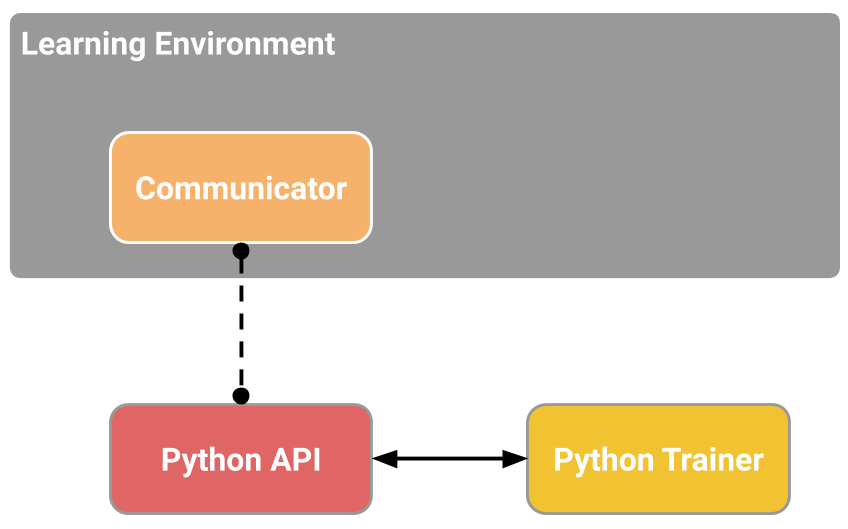
\includegraphics[width = 0.5\textwidth]{Bilder/ml-agents/learning_environment_basic.png}
    \caption{Vereinfachtes Block-Diagramm des ML-Agents-Toolkits \cite{mlagentsOverview}}
    \label{fig:learning-environment-basic}
\end{figure}

Die Trainingsumgebung wird durch zwei enthaltene Unity-Komponenten organisiert \cite{mlagentsOverview}.
\begin{itemize}
    \item \textbf{Agents} sind an ein Unity GameObject geknüpft (beliebiger Charakter innerhalb einer Szene).
    Sie sind gleichzusetzen mit dem Agent eines Reinforcement Learning Problems.
    Agents generieren die Observations (Beobachtungen) des GameObjects, welche dem Reinforcement Learning Algorithmus zugeführt werden, führen die vom Algorithmus empfangenen Aktionen aus und weisen den Reward zu.
    Jeder Agent ist mit einem Behavior verknüpft.

    \item \textbf{Behaviors} (Verhalten) definieren Attribute des Agenten, so auch die Anzahl der Aktionen, die der Agent entgegennehmen kann.
    Ein Behavior kann als Funktion verstanden werden, welche Observations und Reward des Agents als Eingabeparameter enthält und auszuführende Aktionen zurückliefert.
    Behaviors werden in drei Typen unterschieden: \emph{Learning}, \emph{Heuristic} und \emph{Inference}.
    Learning Behaviors sind noch nicht definiert, können aber trainiert werden.
    Heuristic Behaviors werden mittels manuell implementierter Regeln im Quellcode definiert.
    Inference Behavior werden von trainierten Neural-Network-Dateien (entsprechen der finalen, trainierten Policy) repräsentiert.
    Nachdem ein Learning Behavior trainiert wurde, wird es zum Inference Behavior.
\end{itemize}
Herausstellenswert hierbei ist, dass ML-Agents die Möglichkeit bietet, mehrere Agents in einer Trainingsumgebung zu platzieren, die jedoch mit demselben Behavior verknüpft sein können.
Dies kann dafür genutzt werden, das Training zu parallelisieren und damit zu beschleunigen.

\subsection{Reinforcement Learning Algorithmen}
Von ML-Agents werden zwei Trainingsalgorithmen bereitgestellt, die sich dem (Deep) Reinforcement Learning zuordnen lassen.
Dies sind \acf{ppo} und \acf{sac} \cite{mlagentsOverview}.
In \cite{waidner.2020} wurden diese Algorithmen bereits verglichen.
\ac{ppo} ist der Standardalgorithmus von ML-Agents, da er sich, verglichen mit vielen anderen Reinforcement Learning Algorithmen, als für den allgemeinen Einsatz besser geeignet gezeigt hat \cite{schulman2017proximal,openaiPPO}.
\ac{ppo} ist ein on-policy Algorithmus.
Das bedeutet, dass in jeder Iteration des Lernvorgangs nur aus Erfahrungen gelernt wird, die mit der aktuellen Version der Policy gesammelt wurden.
\ac{sac} hingegen ist ein off-policy Algorithmus und lernt somit aus allen Erfahrungen, die er jemals während des gesamten Trainingsvorgangs gesammelt hat \cite{suran2020,sagar2020}.
Daraus ergeben sich für beide Algorithmen unterschiedliche Vor- und Nachteile.
On-policy Algorithmen haben in der Regel einen deutlich stabileren Lernfortschritt, als off-policy Algorithmen.
Andererseits brauchen on-policy Algorithmen in der Regel deutlich mehr Trainingsschritte, um nennenswerte Ergebnisse zu erzielen \cite{mlagentsOverview}.
Im Zuge der Vorgängerarbeit wurde mit beiden Algorithmen gearbeitet, mit dem Ergebnis, dass der \ac{ppo}-Algorithmus auch für das konkrete Problem im Rahmen dieser Studienarbeit deutlich bessere Resultate liefert \cite[48]{waidner.2020}.

\subsection{Training und Hyperparameter}
\label{sec:training}
Wenn die Trainingsumgebung erstellt ist, kann mit dem Training der Agenten begonnen werden.
Der Einstiegspunkt hierzu ist immer die \ac{cli} \code{mlagents-learn}, welche Teil der Python-Umgebung von ML-Agents ist.
Das Training kann dann entweder direkt im Unity-Editor oder mittels einer kompilierten Umgebung erfolgen.
Falls letztere verwendet werden soll, kann sie mittels des Parameters \code{--env=<env\_name>} spezifiziert werden.
Einem Trainingsdurchlauf sollte in der Regel auch ein Run-Identifier zugewiesen werden (\code{--run-id=<run-identifier>}).
Über diesen können die Ergebnisse besser zugeordnet werden und es ist beispielsweise auch möglich, ein unterbrochenes Training wiederaufzunehmen \cite{mlagentsTraining}.

Optional kann das Training mithilfe einer YAML-Datei konfiguriert werden.
In dieser können sowohl allgemeine Aspekte des Trainingsvorgangs festgelegt werden (etwa wie viele Trainingsschritte durchgeführt werden sollen), als auch Hyperparameter eingestellt werden, die spezifisch für das jeweils durchzuführende Training sind.
Für ein Training mit dem \ac{ppo}-Algorithmus sind vor allem die folgenden Hyperparameter von Bedeutung \cite{mlagentsHyperparameter}:
\begin{itemize}
    \item \textbf{batch\_size:} Anzahl der Erfahrungen in jeder Iteration des Gradientenabstiegs.
    \item \textbf{buffer\_size:} Anzahl der Erfahrungen, die gesammelt werden, bevor das Policy-Modell aktualisiert wird, also wie viele Erfahrungen gesammelt werden, bevor gelernt wird.
    \item \textbf{learning\_rate:} Initiale Lernrate für den Gradientenabstieg.
    Damit kann gesteuert werden, wie schnell das Modell am Anfang lernt.
    Sollte so groß wie möglich gewählt werden, um ein schnelles Training durchzuführen.
    Wenn das Training jedoch instabil verläuft, sollte dieser Wert verringert werden.
    \item \textbf{learning\_rate\_schedule:} Gibt an, wie die Lernrate über die Zeit verändert wird.
    Für \ac{ppo} wird diese in der Regel linear verringert, damit das Training möglichst stabil konvergiert.
    \item \textbf{beta:} Faktor um die Entropie des Trainingsprozesses zu regulieren.
    Die Entropie sollte gegenläufig zum Reward langsam im Laufe des Trainingsprozesses fallen.
    Mit einer Erhöhung des beta-Werts wird die Entropie länger auf einem höheren Level gehalten und umgekehrt.
    \item \textbf{epsilon:} Begrenzt die Veränderung der Policy während des Trainingsprozesses.
    Wird epsilon klein gewählt, so werden Änderungen an der Policy kleinschrittiger vorgenommen, was das Training stabilisiert, aber auch mehr Trainingsschritte benötigt.
    \item \textbf{lambd:} Parameter zur Regularisierung während der Berechnung des \enquote{Generalized Advantage Estimate}.
    Prinzipiell gibt der Parameter an, wie stark der Agent auf seine aktuelle Schätzung des Values aufbaut, während die Schätzung des Values aktualisiert wird.
    Bei einem niedrigen Wert von lambd liegt das Gewicht beim aktuell geschätzten Value (der einen hohen Bias haben kann) und bei einem hohen Wert werden die eigentlichen Rewards höher gewichtet (welche jedoch einer hohen Varianz unterliegen können).
    \item \textbf{num\_epoch:} Wie viele Durchläufe durch die gesammelten Erfahrungen gemacht werden können, wenn ein Gradientenabstieg durchgeführt wird.
    Ein kleiner Wert führt zu stabilerem, aber auch langsamerem Training.
    \item \textbf{gamma:} Diskontinuierungsfaktor für zukünftige Rewards.
    Gibt an, wie weit der Agent bei Spekulation auf mögliche Rewards in die Zukunft \enquote{denken} soll.
    \item \textbf{hidden\_units:} Anzahl der Neuronen in den Hidden Layers des zu trainierenden Neural Network.
    Sollte mit der Komplexität des Problems nach oben skaliert werden.
    \item \textbf{num\_layers:} Anzahl der Hidden Layers des Neural Networks.
    Analog zur Anzahl der Neuronen sollte dieser Wert mit der Komplexität des Problems skaliert werden.
    Weniger Layer trainieren in der Regel schneller, können aber unter Umständen zur Abbildung komplexer Probleme nicht ausreichen.
    \item \textbf{normalize:} Gibt an, ob die eingegebenen Observation Vektoren normalisiert werden.
    Bei Problemen mit komplexen, kontinuierlichen Beobachtungs- und Aktionsräumen kann dies hilfreich sein.
\end{itemize}

Die in der Regel verwendeten Befehle zur Initiierung des Trainings folgen grundlegend folgendem Aufbau \cite{mlagentsTraining}: \\
\code{mlagents-learn <yaml-config> --env=<env\_name>  --run-id=<run-id>}

\subsection{Bewertungskriterien}
\label{sec:bewertung}
Der Verlauf des Trainings kann mittels des Tools \emph{Tensorboard} überwacht werden.
Tensorboard startet dabei einen lokalen Webserver, der Auswertungen der Trainingsdaten im Browser darstellt.
Um das Ergebnis eines Trainings objektiv zu bewerten, muss natürlich das eigentliche, resultierende Modell betrachtet werden, jedoch geben auch einige der in Tensorboard dargestellten Metriken frühzeitig Aufschluss über einen potenziellen Erfolg des Trainings.
Allen voran steht der \emph{Cumulative Reward}.
Dieser Wert gibt den mittleren kumulierten Reward innerhalb einer Episode von allen Agenten an.
Natürlich hängt der Verlauf dieser Kurve stark davon ab, wie die individuelle Reward-Funktion gewählt wird, allerdings sollte sich dieser Wert bei einem erfolgreichen Training stetig erhöhen und keine starken Schwankungen aufweisen.
Die \emph{Episodenlänge} zeigt an, wie lange die Episoden im Mittel gedauert haben.
Wird die Umgebung etwa beim unwiderruflichen Scheitern eines Agents zurückgesetzt, so kann hier abgelesen werden, wie lange es im Mittel dauert, bis es zu einem fatalen Scheitern kommt.
\emph{Policy Loss} hängt davon ab, wie stark die Policy sich verändert.
Der Betrag dieser Funktion sollte im Laufe des Trainings abnehmen, wenn die Policy zu einer stabilen Funktion konvergiert.
Schließlich gibt \emph{Value Loss} an, wie stark die vorhergesagten Values von den tatsächlich erhaltenen Rewards abweichen.
Bei einem erfolgreichen Training sollte dieser Wert zu Beginn ansteigen und dann im Anschluss gegen einen niedrigen Wert konvergieren \cite{aurelian2018,untiyMetrics}.

Weiterhin werden in Tensorboard die Hyperparameter im Laufe der Zeit dargestellt.
Entsprechend den Beschreibungen in \autoref{sec:training} können auch diese Werte live mitverfolgt und gegebenenfalls korrigiert werden.


\section{Vektorgeometrie}
Da Vektoren im dreidimensionalen Raum ein essenzieller Bestandteil der Arbeit mit Unity sind, werden die dafür wichtigen Konzepte hier kurz vorgestellt.

Grundsätzlich gesehen ist ein Vektor ein mathematisches Konstrukt und hat eine Länge und eine Richtung.
Im Gegensatz zu Punkten geben Vektoren keinen festen Ort an, sondern beschreiben den Weg von einem Punkt zu einem anderen \cite[6]{kohn2012}.
Dabei besitzt ein Vektor für jede Dimension eine Komponente.
Trotzdem ist eine Ortsangabe mit einem Vektor möglich (und wird in Unity für die GameObjects verwendet).
Dieses Konstrukt besteht aus einem Vektor, der an einem bestimmten Punkt beginnt und nennt sich Ortsvektor \cite[21]{kohn2012}.
Im weiteren Verlauf wird davon ausgegangen, dass Ortsvektoren dem Koordinatenursprung entstammen.

\autoref{fig:weg} stellt die Ortsvektoren $\overrightarrow{a}$ und $\overrightarrow{b}$ dar, welche vom Koordinatenursprung auf die Punkte $A$ und $B$ zeigen.
Der Vektor $\overrightarrow{AB}$ stellt den Vektor dar, der von $A$ zu $B$ führt.
Addiert man mehrere Vektoren, so erhält man den daraus resultierenden Vektor \cite[11]{kohn2012}.
Wie in \autoref{eqn:weg} ersichtlich ist, kann durch Addition von $\overrightarrow{a}$ und $\overrightarrow{AB}$ wiederum $\overrightarrow{b}$ bestimmt werden.
Mittels eines Umstellens der Gleichung kann aber auch aus den beiden Ortsvektoren der Verbindungsvektor $\overrightarrow{AB}$ bestimmt werden \cite[12]{kohn2012}.

\begin{figure}
    \centering
    \begin{tikzpicture}
        \coordinate[label=right:$A$] (A) at (3,2.5);
        \coordinate[label=left:$B$] (B) at (2,5);

        \draw[-latex] (0,0) -- node[below] {$\overrightarrow{a}$} (A);
        \draw[-latex] (0,0) -- node[left] {$\overrightarrow{b}$} (B);
        \draw[-latex, dashed] (A) -- node[right] {$\overrightarrow{AB}$} (B);
    \end{tikzpicture}
    \caption{Vektor von Punkt $A$ zu Punkt $B$}
    \label{fig:weg}
\end{figure}

Für die Länge eines Vektors (auch Norm genannt), gibt es verschiedene Definitionen.
Die hier relevante und erklärte ist die sogenannte \emph{euklidische Norm}.
Zur Bestimmung dieser wird die Summe aus den Quadraten der Komponenten gebildet und aus dieser Summe im Anschluss die Quadratwurzel gezogen \cite[30]{kohn2012} (\autoref{eqn:laenge3d}).
Der Hintergrund liegt hierbei im Satz des Pythagoras, was ersichtlich wird, wenn man sich die Zerlegung eines zweidimensionalen Vektors in seine einzelnen Komponenten anschaut (\autoref{fig:zerlegung}, \autoref{eqn:laenge2d}).


\begin{equation}
    \label{eqn:weg}
    \overrightarrow{a} + \overrightarrow{AB} = \overrightarrow{b}
    \quad \Rightarrow \quad
    \overrightarrow{AB} = \overrightarrow{b} - \overrightarrow{a}
\end{equation}

\begin{figure}
    \centering
    \begin{tikzpicture}
        \draw[-latex, dashed] (0,0) -- node[below] {$\overrightarrow{x}$} (5,0);
        \draw[-latex, dashed] (5,0) -- node[right] {$\overrightarrow{y}$} (5,5);
        \draw[-latex] (0,0) -- node[left] {$\overrightarrow{v}$} (5,5);
    \end{tikzpicture}
    \caption{Zerlegung des zweidimensionalen Vektors $\overrightarrow{v}$}
    \label{fig:zerlegung}
\end{figure}

\begin{equation}
    \label{eqn:laenge2d}
    \overrightarrow{v} = \begin{pmatrix}x \\ y\end{pmatrix}
    \quad \Rightarrow \quad
    |\overrightarrow{v}| = \sqrt{x^2 + y^2}
\end{equation}

\begin{equation}
    \label{eqn:laenge3d}
    \overrightarrow{v} = \begin{pmatrix}x \\ y \\ z\end{pmatrix}
    \quad \Rightarrow \quad
    |\overrightarrow{v}| = \sqrt{x^2 + y^2 + z^2}
\end{equation}

Dadurch, dass Vektoren eine Richtung darstellen, ist es ebenfalls möglich, den Winkel $\beta$ zu bestimmen, der zwischen diesen Vektoren liegt, wenn man sie aufeinander stellt.
Dafür wird zunächst das sogenannte Skalarprodukt der beiden Vektoren gebildet \cite[45]{kohn2012} (\autoref{eqn:skalarprodukt}).
Anschließend wird das Skalarprodukt durch das Produkt der Längen beider Vektoren geteilt und in die $\arccos$-Funktion eingesetzt \cite[60]{kohn2012} (\autoref{eqn:zwischenwinkel}).

\begin{equation}
    \label{eqn:skalarprodukt}
    \overrightarrow{v} \cdot \overrightarrow{w} =
    \begin{pmatrix}v_1 \\ v_2 \\ v_3\end{pmatrix} \cdot \begin{pmatrix}w_1 \\ w_2 \\ w_3\end{pmatrix} =
    v_1 \cdot w_1 + v_2 \cdot w_2 + v_3 \cdot w_3
\end{equation}

\begin{equation}
    \label{eqn:zwischenwinkel}
    \beta = \arccos(\frac{\overrightarrow{v} \cdot \overrightarrow{w}}{|\overrightarrow{v}| \cdot |\overrightarrow{w}|})
\end{equation}


\section{Beschreibung der Projektbasis}
Die Zielsetzung dieser Arbeit soll aufbauend auf einer Vorgängerarbeit \cite{waidner.2020} realisiert werden, welche vor einigen Jahren ebenfalls im Rahmen einer Studienarbeit durchgeführt wurde.
Hier soll zunächst die Vorgehensweise der Vorgängerarbeit in ihren Grundzügen erläutert werden.

\subsection{Aufbau und Simulation des Roboters}
Kernelement der Arbeit ist ein vierbeiniger, 3D-gedruckter Roboter, der in seiner Anatomie einer Spinne gleicht.
Der Roboter besteht aus einer rechteckigen Zentralplatte.
An jeder Ecke dieser Platte ist ein Bein angebracht.
Die Beine des Roboters bestehen jeweils aus drei separaten Teilen.
Folglich hat jedes Bein zwei Gelenke \cite[52]{waidner.2020}.
Jedes dieser Gelenke wird mit einem Servomotor des Typs SG90 XY realisiert, welche sich in einem Aktionsradius von 180° bewegen können.
Die Neutralstellung der Beine ist die jeweilige Mittelposition des Servomotors.
Angegeben wird der Aktionsradius des Servos als Wert im Bereich 0° - 180°, die Mittelstellung befindet sich also bei 90° \cite[38]{waidner.2020}.
Die verwendeten Servomotoren bewegen sich nur auf einer Achse.
An der Stelle, an der die Beine mit dem Körper verbunden sind, befindet sich ein weiterer Servomotor.
Mithilfe der verbauten Servomotoren ist es möglich, jedes Bein anzuziehen oder auszustrecken und es nach vorne beziehungsweise hinten zu bewegen.

Angesteuert werden die Servomotoren mit einem ESP8266 Mikrocontroller, welcher mittels I²C Steuersignale an ein Servo-Breakout-Board sendet, an welchem wiederum die Servomotoren angeschlossen sind.
Die Stromversorgung erfolgt über eine Batterie, damit sich der Roboter autark von einer Stromquelle im Raum bewegen kann \cite[54]{waidner.2020}.
Die aufgelisteten Bauteile werden so mit Kabelbindern an der Zentralplatte befestigt, dass sie nicht mit der Bewegungsfreiheit der Beine interferieren.
Am Roboter ist keinerlei Sensorik verbaut \cite[36]{waidner.2020}.

Da das Training des Roboters in der Realität zu lange dauert und dabei außerdem die Gefahr droht, den Roboter zu beschädigen, wurde eine Simulationsumgebung aufgebaut, in der das Training des Roboters erfolgt.
Diese ist in Unity realisiert.
In Unity ist es möglich, dasselbe 3D-Modell zu importieren, das auch für den Druck der Teile des Roboters verwendet wird, was eine akkurate Umsetzung der Dimensionen sicherstellt.

Die größte Schwierigkeit einer Simulation des Roboters besteht darin, die Servomotoren abzubilden.
Im Gegensatz zu einem Computerprogramm ist es Bauteilen in der realen Welt nicht möglich, instantan einen gezielten Zustand anzunehmen.
Das heißt, wird für einen Servomotor ein neuer Winkel vorgegeben, so braucht dieser eine bestimmte Zeit, bis er diesen erreicht hat.
Diese Zeit ist einerseits von der Bewegungsgeschwindigkeit des Servomotors abhängig, andererseits stellt die Last, die der Motor bewegt, einen weiteren Einflussfaktor dar.
Die Vorgängerarbeit implementiert eine Software-Simulation der Servomotoren, bei denen zumindest der Aspekt der mittleren Bewegungsgeschwindigkeit berücksichtigt wird, sowie verwandte, allgemeine Charakteristika der Bewegung \cite[37]{waidner.2020}.
Zusätzlich werden in Unity die ungefähren Gewichte der einzelnen Teile eingetragen, um eine akkurate Simulation der physikalischen Kräfte zu ermöglichen, die auf den Roboter einwirken.
Die Simulation dieser allgemeinen Physik wird bereits als Grundfunktion der Unity-Engine bereitgestellt und muss nicht separat implementiert werden.

% \begin{itemize}
%     \item Roboter aus 3D gedruckten Teilen
%     \item 4 Beine mit 2 Teilen, d.h. 2 Gelenken pro Bein, eins im Bein und eins am Körper
%     \item Gelenke sind Servos mit 120° Aktionsradius
%     \item Neutralstellung ist Mitte des Servos, also 60°
%     \item Steuerung über ESP8266 und Servo Breakout Board
%     \item Stromversorgung über Batterie
%     \item keine weitere Sensorik
    
%     \item Simulation dieses Roboters in Unity
%     \item dazu direkter Import des 3D Modells
%     \item Software-Simulation der Servos und deren Charakteristika (Bewegungsgeschwindigkeit)
%     \item ungefähres Gewicht der einzelnen Teile hinterlegen für Physiksimulation
% \end{itemize}

\subsection{Training des Roboters}
Mit der fertig aufgebauten Simulation kann der Roboter für alle erdenklichen Szenarien trainiert werden.
Dazu müssen Rahmenbedingungen des Trainings definiert werden.
Primär sind dies die Observations, die der Trainingsalgorithmus macht, die Aktionen, die er ausführen kann und der Reward, den er als Feedback für seine Handlungen erhält.
Die Zielsetzung der Vorgängerarbeit besteht aus einer reinen Vorwärtsbewegung.
Da der reale Roboter über keine Sensorik verfügt und lediglich die Ansteuerwinkel seiner Servomotoren kennt, sind dies auch die einzigen Observations, die dem Algorithmus zugänglich gemacht werden (kontinuierlicher Beobachtungsraum).
Als Aktionen kann der Algorithmus beliebige Zielwinkel für die Servomotoren setzen (kontinuierlicher Aktionsraum).
Der Reward für den Roboter besteht in der Vorgängerarbeit aus der Streckendifferenz, die er nach vorne zurückgelegt hat.
Bestraft wird der Roboter für ein Umkippen, um zu verhindern, dass bei der späteren Übertragung auf den realen Roboter die Steuerelektronik beschädigt wird.
Um das Training zu beschleunigen, sind in der Vorgängerarbeit mehrere Agents nebeneinander in derselben Umgebung instanziiert.
Nach einer Einstellung der Hyperparameter wurden Modelle mit den Reinforcement-Learning-Algorithmen \ac{sac} und \ac{ppo} trainiert.
Dabei wurde festgestellt, dass in diesem Anwendungsfall die Ergebnisse des \ac{ppo}-Algorithmus denen des \ac{sac}-Algorithmus deutlich überlegen sind \cite[48]{waidner.2020}.

Die Bewegungsart, die der Roboter sich bei den vorgegebenen Trainingsbedingungen antrainiert, ist keine klassische Form des natürlichen Laufens.
Stattdessen führen die Ergebnisse des Trainings dazu, dass der Algorithmus den Roboter mit einem der Hinterbeine einknicken lässt und ihn dann sprungartig nach vorne katapultiert \cite[51]{waidner.2020}.

\subsection{Übertragung in die Realität}
Die Implementierung der Vorgängerarbeit sieht auch eine Übertragung der Ergebnisse auf den realen Roboter vor.
Zu diesem Zwecke können die Steuersignale, die der Roboter in der Simulation erhält, über eine serielle Verbindung übertragen und direkt auf dem realen Roboter angewandt werden.

Die unternommenen Versuche waren jedoch leider nicht erfolgreich.
Als Ursache fällt die Vermutung auf Hardwarefehler, da der Roboter -- in der Luft gehalten -- die Bewegungen korrekt nachahmt.
Wird der Roboter jedoch auf den Boden gestellt, knickt er unter seinem Gewicht sofort ein und kann die gelernte Laufmethodik nicht anwenden \cite[58]{waidner.2020}.

\chapter{State of the Art}


\begin{itemize}
    \item \enquote{Decentralized Deep Reinforcement Learning for a Distributed and Adaptive Locomotion Controller of a Hexapod Robot}
    \item Machine Learning in letzten Jahren erfolgreich auf viele Aufgaben angewandt
    \item DRL scheint noch Probleme zu haben bei der Anwendung für reale Roboter in \enquote{continuous control tasks}
    \item vor allem im Umgang mit unvorhergesehenen Situationen gibt es Probleme
    
    \item ursprünglich aus Bereich Computerspiele, deshalb viel in simulierten Umgebungen
    \item Transfer auf reale Probleme kann schwierig sein (\enquote{nature of such problems is fundamentally different from those in playing computer games})
    \item häufig wird zunächst die Simulation genutzt, um Grundsteine zu legen, die dann manuell feingeschliffen werden für eine bestimmte Aufgabe
    \item zwei fundamentale Probleme: soll den Reward ausnutzen, neigt deshalb zu Overfitting; reale Anwendungen deutlich mehr (Signal-)Rauschen, führt zu Hinterfragen von festem Markov Decision Process
    \item DRL tendiert dazu, Nischenlösungen zu finden, die meist nicht dazu in der Lage sind, adaptiv auf neue Situationen zu reagieren
    
    \item Tendenz geht dahin, hierarchische oder dezentralisierte Ansätze zu verfolgen
    \item hierarchisch erlaubt flexibles wechseln zwischen verschiedenen Unteraufgaben und Verhaltensweisen und somit auch Agieren in verschiedenen Kontexten möglich, bislang allerdings nur mit geringen Freiheitsgraden umgesetzt
    \item Fokus diesen Papers eher auf Störungen und Varietät in einem spezifischen Kontext mit einem spezifischen Verhalten
    
    \item PPO funktioniert allgemein gut mit kontinuierlichen Problemen ohne viel Hyperparameter-Tuning
    \item Median-Geschwindigkeit einer Episode ist der Reward
    \item \cite{schilling2020decentralized}
\end{itemize}

\begin{figure}
    \centering
    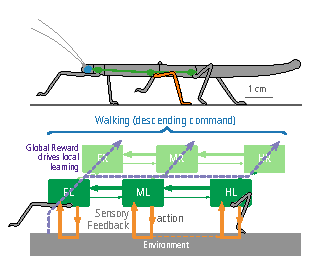
\includegraphics[width = 0.35\textwidth]{Bilder/decentralized-insect.pdf}
    \caption{\cite{schilling2020decentralized}}
\end{figure}


\hrule
\begin{itemize}
    \item \enquote{Adaptation of a Decentralized Controller to Curve Walking in a Hexapod Robot}
    \item bei Robotern mit mehreren Beinen aktuell drei vorherrschende Ansätze
    - Central Pattern Generators (CPGs)
        - Oszilatorsysteme oder neurale Netze, die rhythmische Ausgabe erzeugen, ohne bestimmte Eingabe vorauszusetzen
    - lernende Ansätze
    - Sensorenbasierte Ansätze
        - sind besser erklärbar verglichen mit lernenden Ansätzen
        - normalerweise relativ anpassbar an sich verändernde Umgebungen
    
    \item sehen Potenzial in Verbindung mehrerer Ansätze
    \item \cite{simmering2023walknet}
\end{itemize}


\hrule
\begin{itemize}
    \item \enquote{DeepGait: Planning and Control of Quadrupedal Gaits using Deep Reinforcement Learning}
    \item Kombination von state-of-the-art modellbasierten Methoden der Bewegungsplanung und Reinforcement Learning
    \item Evaluieren die physikalische Machbarkeit anstatt physisch zu simulieren
    \item trennen Schrittplanung und Ausführung
    \item es können ganze Schritte evaluiert werden und nicht nur einzelne Frames einer Simulation
    \item Hauptproblem in Schrittplanung ist Kombinatorik, wegen der vielen möglichen Kombinationsmöglichkeiten für Kontaktpunkte mit dem Untergrund
    \item aber: Training auf späterem Terrain, allerdings relativ gute Verallgemeinerung
    \item Entropie ist extrem wichtig
    \item Weit bessere Resultate als andere Ansätze, gerade was das Überbrücken von Klüften angeht
    \item \cite{tsounis2020deepgait}
\end{itemize}


\hrule
\begin{itemize}
    \item \enquote{Learning and Adapting Agile Locomotion Skills by Transferring Experience}
    \item selbst einfache Aufgaben können sehr komplexe modulierte Reward-Funktionen benötigen, um die gezielten Bewegungen zu erhalten
    \item Wenn eine Bewegungsform sehr gut koordinierte Bewegungen voraussetzt, kann sehr schwer sein, wenn man von Null beginnt (-> nur sehr konkretes Verhalten kann Reward nach sich ziehen)
    \item Für ein spezifisches Zielproblem zu trainieren mag schwer sein, doch häufig ist es möglich, mit einfacheren Trainingsumgebungen zumindest relevante Daten zu erhalten, welche für einen Lernprozess von Interesse sind
    \item (Aus auf Hinterbeinen stehen wird Laufen)
    \item Häufig ist es schwierig, das in agileres Verhalten zu erweitern; insbesondere mit stark angepassten Reward-Funktionen, um das Verhalten überhaupt erst zu erzeugen
    \item => Training Agiler Roboter Fähigkeiten erleichtern durch Transfer mit existierenden suboptimalen Fähigkeiten
    \item \cite{smith2023learning}
\end{itemize}

\begin{figure}
    \centering
    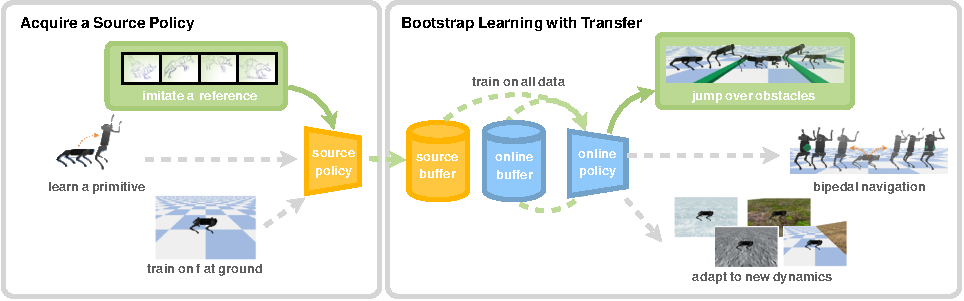
\includegraphics[width = \textwidth]{Bilder/transfer-learning.pdf}
    \caption{\cite{smith2023learning}}
\end{figure}
\chapter{Konzeptionierung}
\section{Einschränkungen und Übertragungsprobleme}
\label{sec:probleme}
In der Vorgängerarbeit sollte der Roboter bislang nur geradeaus laufen.
Dabei verfügt der verwendete Roboter über keinerlei Sensorik.
Einzig die aktuellen Zielwinkel der Servomotoren, welche die Bewegung der Beine ermöglichen, sind dem Lernalgorithmus zugänglich.
Das Training des Roboters erfolgte jedoch rein in der Simulation.
Da die Simulationsumgebung nicht nur den Roboter, sondern dessen komplettes Umfeld abbilden muss, sind alle Informationen, die ein beliebiger Sensor liefern könnte theoretisch in der Simulation vorhanden, wurden dem Algorithmus jedoch nicht zugänglich gemacht.
Der Roboter kennt seinen eigenen Zustand nicht, beziehungsweise nur bedingt.
Das trainierte Modell wird lediglich in der Praxis angewandt, unter der Annahme, dass bei einem korrekt gelernten Modell keinerlei Zusatzinformationen notwendig sind, um den Roboter seine Aufgabe erfüllen zu lassen: geradeaus zu laufen.

Die Zielsetzung dieser Studienarbeit erweitert nun jedoch diese Aufgabe des Roboters, was Probleme aufwirft.
Der Roboter soll lernen, einem vorgegebenen Pfad zu folgen.
Dabei soll der Pfad für jeden Durchlauf dem Roboter individuell vorgegeben werden können.
Besonders wichtig ist hierbei zu beachten, dass der Roboter unter keinen Umständen einen bestimmten Pfad auswendig lernen soll, denn dann müsste für jeden Pfad, den der Roboter laufen soll, ein eigenständiges Modell trainiert werden, was einen praktischen Nutzen unmöglich machen würde -- schließlich kann nicht für eine Bewegungsanweisung an einen Roboter jedes Mal mehrere Stunden Rechenzeit aufgebracht werden.
Dem Roboter muss also ein Pfad mitgegeben werden.
Außerdem muss für das Training des Roboters mehrfach dieser übergebene Pfad neu generiert werden, um ein Auswendiglernen zu verhindern.

Dass der Roboter einem frei angegebenen Pfad folgen können soll, wirft die Frage auf, ob er dazu Informationen über seine Position im Raum benötigt.
Rein theoretisch betrachtet könnte diese Frage einfach mit \enquote{Nein} beantwortet werden.
Prinzipiell gesehen kann der Roboter seine aktuelle Position anhand seiner vergangenen Bewegungen vom Ausgangspunkt her berechnen.
Andererseits würde dies eine enorm hohe Präzision der Bewegungen voraussetzen.
Außerdem könnte der Roboter in der Realität auf dem Boden rutschen.
Auch läuft das bisherige Modell -- nicht einmal in der Simulation -- verlässlich geradeaus, sondern hat dabei immer einen leichten Drall zur Seite.
Aus diesen Gründen wird der Schluss gezogen, dass durch minimale, nicht vermeidbare Abweichungen die Ausführung der Aufgabe nur sehr ungenau möglich wäre, wenn keine Positionierungsinformationen zur Verfügung gestellt werden.

In der Simulation gestaltet sich eine mögliche Lösung des Problems sehr einfach: Der Roboter ist ein Game-Objekt innerhalt der Unity-Engine.
Als solches besitzt er automatisch Koordinaten innerhalb der Simulation, welche einfach für den Roboter freigegeben werden können.
Bei einer späteren Übertragung in die Realität können diese Informationen durch andere, konkrete Ortungssysteme geliefert werden.
Es wäre lediglich ein Mapping erforderlich, um das Informationsformat eines konkreten Sensors in das Koordinatenformat von Unity umzuwandeln.
Diese Informationen können dann dem Modell für die Inferenz zur Verfügung gestellt werden.
Somit ist es möglich, ein Modell zu trainieren, welches unabhängig von der später eingesetzten Ortungstechnologie ist.

Weiterhin umfasst die Aufgabenstellung, dass der Roboter Hindernisse auf seinem Weg erkennen und gezielt umgehen können soll.
Anschließend soll er auf den vorgegebenen Pfad zurückkehren, wobei die Abweichung möglichst gering ausfallen sollte.
Hierfür wird eine Hindernis- beziehungsweise Kollisionserkennung benötigt.
Mit der aktuellen technischen Ausstattung des Roboters ist auch diese Aufgabe nicht umsetzbar.
In der Simulation soll vereinfacht für die Hinderniserkennung die Kollisionserkennung der Beine verwendet werden.
(Diese Kollisionserkennung kann Unity für sämtliche Game-Objekte durchführen.)
Dadurch muss der Roboter mit seinem Hindernis zusammenstoßen, um es wahrzunehmen.
In der Realität wäre natürlich eine Hinderniserkennung sinnvoll, mit der Hindernisse bereits vor einer Kollision erkannt werden können (zum Beispiel LiDAR, Kameras oder ähnliche Systeme).

Sowohl für die Ortung, als auch für die Hinderniserkennung wäre in der Realität der Einsatz komplexer Systeme nötigt.
Die Integration solcher würde jedoch den Umfang dieser Arbeit erheblich übersteigen.
Hier soll eher ein Proof-of-Concept für die selbstständige Umsteuerung von Hindernissen erarbeitet werden.
Es soll keine Übertragung der in der Simulation trainierten Modelle auf den realen Roboter stattfinden.

Die Springbewegung, die der Roboter sich bislang antrainiert hat, führt zu weiteren potenziellen Problemen.
Zwar wurde, wie oben beschrieben, der Einsatz eines Ortungssystems festgelegt, jedoch bringt diese Bewegungsform trotzdem massive Genauigkeitsprobleme mit sich. 
Sie ist sehr kraftaufwändig und instabil, der Roboter schwankt dabei stark um seine horizontale Achse und kann seine exakte Landeposition nur bedingt steuern.
Da der Roboter Hindernisse über eine Kollision mit diesen erkennen soll, würde außerdem das Problem bestehen, dass der Roboter im Sprung gegen diese knallen könnte.
Aus den genannten Gründen ist es sinnvoll, Maßnahmen zur Einschränkung der Bewegung des Roboters vorzunehmen.
Möglich wäre zum Beispiel eine Anpassung der Belohnungsfunktion, wonach starke Höhenänderungen oder Neigungen der Zentralplatte des Roboters bestraft werden.

% \begin{itemize}
%     \item bislang sollte der Roboter nur geradeaus laufen
%     \item Roboter verfügt über keinerlei Sensorik
%     \item kennt nur den aktuellen Winkel der Beine/Servomotoren
%     \item Training erfolgte rein in der Simulation
%     \item die Simulationsumgebung kennt den Zustand (z.B. Neigung) des Roboters und kann anhand dessen den Wert der Belohnungsfunktion berechnen und an den Roboter zurückmelden
%     \item Roboter kennt seinen eigenen Zustand nicht
%     \item bisheriges Modell wird lediglich in der Praxis angewandt, unter der Annahme, dass bei korrekt gelerntem Modell keinerlei Zusatzinformationen notwendig sind, um den Roboter seine Aufgabe erfüllen zu lassen: geradeaus zu laufen
% \end{itemize}

% Probleme in der erweiterten Aufgabenstellung:
% \begin{itemize}
%     \item der Roboter soll nun einem vorgegebenen Pfad folgen
%     \item dabei soll der Pfad für jeden Durchlauf dem Roboter individuell vorgegeben werden können
%     \item der Roboter soll NICHT einen vorgegebenen Pfad lernen und danach immer von diesem Pfad ausgehen
%     \item dem Roboter muss also ein Pfad mitgegeben werden können
    
%     \item Positionierungsinformationen benötigt?
%     \item einerseits nein, theoretisch kann der Roboter seine aktuelle Position anhand seiner vergangenen Bewegungen vom Ausgangspunkt bestimmen
%     \item andererseits ja, da der Roboter auf dem Boden rutschen kann (zumindest in der Realität), das Berechnen von Entfernungen den gesamten Algorithmus stark verkompliziert und unter Umständen durch kleinere Abweichungen sehr ungenau ausfallen kann
%     \item mögliche Lösung in der Simulation: Positionierungsinformationen innerhalb der Simulationsumgebung für Roboter freigeben
%     \item diese Informationen könnten dem Roboter später durch andere Sensoren geliefert werden
%     \item wenn das Informationsformat des neuen Sensors umgewandelt wird in das bisherige Format (zum Beispiel durch ein externes Modul), könnte ein anderer Sensor Plug-And-Play in das trainierte Modell integriert werden
    
%     \item außerdem soll der Roboter Hindernisse auf seinem Weg erkennen und gezielt umgehen können
%     \item danach soll auf den Pfad zurückgekehrt werden
%     \item dafür wird eine Hindernis-/Kollisionserkennung benötigt
%     \item aktuell hat der Roboter keinerlei solche Sensorik
%     \item vereinfacht soll für die Hinderniserkennung in der Simulation die Kollisionserkennung für die Beine verwendet werden
%     \item dadurch muss der Roboter mit seinem Hindernis zusammenstoßen, um es wahrzunehmen
%     \item in der Realität wäre natürlich eine Hinderniserkennung sinnvoll, mit der Hindernisse bereits vor einer Kollision erkannt werden können (z.B. LiDAR, Kameras oder ähnliche), die Integration solcher Systeme würde jedoch den Umfang dieser Arbeit erheblich übersteigen
%     \item hier soll eher ein Proof-of-Concept für die selbstständige Umsteuerung von Hindernissen erarbeitet werden
    
%     \item Genauigkeitsprobleme beim Übertragen der Springbewegung: daher genauere Einschränkungen für den Algorithmus
%     \item bisher bewegt sich der Roboter nach Training in einer springenden Bewegung fort
%     \item diese Bewegungsform ist sehr kraftaufwändig und instabil, der Roboter schwankt dabei stark um die horizontale Achse und kann seine exakte Landeposition nur bedingt steuern
%     \item vor allem relevant, falls dem Roboter keine Positionierungsinformationen zur Verfügung gestellt würden, da dann jeder Millimeter zählt
%     \item aber auch zur Erhöhung der allgemeinen Genauigkeit und Reduzierung der Fehler, wäre es sinnvoll, die Fortbewegung des Roboters zu stabilisieren
%     \item mögliche Maßnahme zur Einschränkung der Bewegung: restriktive Anpassung der Belohnungsfunktion, wenn sich die Höhe des Mittelteils des Roboters zu stark verändert oder dieser spürbar die Neigung zum Horizont verändert, wird der Agent bestraft
    
%     \item Insgesamt soll keine Übertragung des implementierten Modells auf den realen Roboter stattfinden
%     \item wie oben beschrieben wäre eine Implementierung von diversen Sensoren vonnöten, was den Umfang dieser Arbeit deutlich übersteigt
% \end{itemize}

\section{Wahl der Simulationsumgebung}
In der Vorgängerarbeit wurden bereits drei mögliche Simulationsumgebungen ausführlich gegenübergestellt \cite[27]{waidner.2020}.
Die beschriebenen Bedingungen haben sich dabei leicht verändert.
Aus dem Vergleich ging hervor, dass MuJoCo aufgrund seiner äußert realistischen Simulation der Physik und einem Fokus auf Gelenksimulation eine gute Wahl für eine Trainingsumgebung wäre.
Jedoch war der Einsatz von MuJoCo damals mit erheblichen Lizenzgebühren verbunden, was einer der Gründe war, diese Software nicht zu verwenden.
Mittlerweile ist MuJoCo allerdings frei und quelloffen verfügbar \cite{mujoco.org,github.mujoco}, was dafür sprechen würde, die Programmwahl neu zu überdenken.

Andererseits soll diese Arbeit an die vorangegangene anknüpfen.
Wenn die Simulationsumgebung gewechselt würde, müsste im Grunde genommen von vorne begonnen werden, da die meisten Aspekte der Vorarbeit, wenn nicht sogar alle, nicht einfach außerhalb der Unity-Umgebung genutzt werden können.
Deshalb wird die Wahl getroffen, weiterhin Unity zu verwenden.
Unity bietet jedoch die Möglichkeit, die standardmäßig verwendete Physics-Engine gegen andere, über Plugins bereitgestellte, auszutauschen.
MuJoCo ist ebenfalls als ein solches Plugin verfügbar \cite{mujocoUnityPlugin}.
Insofern könnte bei Bedarf theoretisch mit geringem Aufwand in Betracht gezogen werden, MuJoCo als Physics-Engine in Unity einzubinden, um somit das Gesamtergebnis des Trainings durch eine bessere Physiksimulation zu verbessern.
Auch wäre es denkbar, die Ergebnisse der verschiedenen Umgebungen zu vergleichen.
Da jedoch keine Übertragung auf einen realen Roboter erfolgt, dürfte in diesem Kontext vermutlich kein spürbarer Unterschied zwischen den Physics-Engines zu beobachten sein.
Selbst falls ein messbarer Unterschied bestehen sollte, könnte dieser nicht hinsichtlich seiner Aussagekraft eingeordnet werden.


% \begin{itemize}
%     \item in der Vorgängerarbeit wurde bereits über verschiedene mögliche Simulationsumgebungen geschrieben
%     \item die Bedingungen haben sich leicht geändert
%     \item eine mögliche Software (MuJoCo) ist mittlerweile nicht mehr kostenpflichtig, was damals einer der Gründe war, die gegen diese Software gesprochen haben
%     \item andererseits soll diese Arbeit an die vorangegangene anknüpfen
%     \item wenn die Simulationsumgebung gewechselt würde, würde man im Grunde genommen kaum Ergebnisse der Vorgängerarbeit aufgreifen sondern in vielen Gesichtpunkten von 0 beginnen
%     \item deshalb soll weiterhin Unity verwendet werden
%     \item Unity bietet jedoch die Möglichkeit, die standardmäßige Physics-Engine gegen andere nach dem Plugin-Prinzip auszutauschen
%     \item insofern könnte realistisch und mit geringem Aufwand in Betracht gezogen werden, MuJoCo als Physics-Engine in Unity einzubinden, um somit das Ergebnis des Trainings durch eine andere/verbesserte Physiksimulation zu verbessern
%     \item auch wäre es möglich, die Ergebnisse der verschiedenen Umgebungen zu vergleichen
%     \item da jedoch keine Übertragung auf einen realen Roboter erfolgt, dürfte in diesem Kontext kein spürbarer Unterschied zu beobachten sein / ein beobachteter Unterschied könnte nicht hinsichtlich seiner Aussagekraft eingeordnet werden
% \end{itemize}

\section{Geplante Realisierung}
Die Umsetzung der Arbeit lässt sich in mehrere Aufgabenpakete gliedern.
Diese sollen folgend beschrieben werden.

\subsection{Rekonstruktion}
Der erste Schritt besteht darin, die Simulationsumgebung und Lernergebnisse der vorherigen Arbeit zu rekonstruieren.
Diese Rekonstruktion bringt Probleme mit sich.
Einige der verwendeten Komponenten sind einer starken Entwicklung unterlegen -- insbesondere das erst 2017 vorgestellte ML-Agents Toolkit, welches sich zum Zeitpunkt der Bearbeitung des Basisprojekts noch in der Pre-Release-Phase befand \cite{mlagentsHistory}.
Deshalb sind auf jeden Fall Änderungen nötig, um die bestehenden Ergebnisse überhaupt sichten zu können.
Außerdem empfiehlt es sich, die Umgebung auf den aktuellen Stand der Technik zu migrieren, um von potenziellen Verbesserungen im verwendeten Tooling profitieren zu können.
Auch wird damit eine zukunftssicherere Basis geboten, auf der die Ergebnisse dieser Arbeit weitergenutzt werden können.

\subsection{Entwurf der Pfadplanung}
Im Anschluss an die Konstruktion einer verwendbaren Simulationsumgebung muss ein Format entworfen werden, wie dem Roboter ein Pfad mitgeteilt werden kann, dem dieser folgen soll.
Ein Pfad besteht aus mathematischer Sicht aus einer geordneten Aufreihung an Punkten.
Der Roboter muss diese der Reihe nach ansteuern.
Wie in \autoref{sec:probleme} bereits ausgeführt, muss verhindert werden, dass der Roboter einen vorgegebenen Pfad auswendig lernt.
Als logische Folgerung muss bei jeder Trainingsepisode ein zufälliger Pfad vorgegeben werden.
Beim Verflogen eines Pfades ist zu jeder Zeit nur der als nächstes anzusteuernde Punkt von Relevanz.
Für das Training ergibt dies Parallelen zu einem Beispielszenario des ML-Agents-Toolkits.
Beim Crawler-Example muss eine Kreatur lernen, ein zufällig spawnendes Ziel (sogenannte \emph{Dynamic Targets}) zu erreichen.
Kommt der Crawler mit einem Dynamic Target in Berührung, teleportiert es sich an einen zufälligen Ort \cite{crawlerExample}.
Dabei tauch die Dynamic Targets als kleine Würfel in der Umgebung des Crawlers auf.
Die Dynamic Targets könnte auch für die Pfadplanung des Roboters verwendet werden.
Die für das Training notwendigen, zufälligen Pfade bilden sie bereits automatisch ab.
Um später einen festen Pfad vorgeben zu können, müsste lediglich eine kleine Modifikation der Dynamic Targets vorgenommen werden, um diese in einer festgelegten Reihenfolge anstatt zufällig erscheinen zu lassen.

\subsection{Anpassung der Belohnungsfunktion}
Bislang wird der Roboter nur für eine zurückgelegte Distanz entlang der x-Achse belohnt und erhält eine Bestrafung, wenn er sich auf den Rücken dreht.
Im ersten Schritt soll das Laufverhalten des Roboters stabilisiert werden, damit sich dieser nicht mehr springend fortbewegt.
Dazu könnte etwa in der Belohnungsfunktion ein Faktor eingebracht werden, der den Roboter mit einem, an der Neigung der Zentralplatte skalierten, Wert bestraft.

Um den Roboter dazu zu bringen, zum nächsten Zielpunkt zu laufen, muss die bisherige Belohnung für die Distanz ersetzt werden.
Denkbar sind hierfür mehrere Ansätze.
Eine Möglichkeit besteht darin, die Distanz zwischen Roboter und Zielpunkt zu bestimmen und mit der Distanz vor der letzten Aktion zu vergleichen.
Die andere Möglichkeit wäre, die konkrete Bewegungsrichtung des Roboters zu bestimmen und ein Produkt mit der Geschwindigkeit zu bilden.
Diese Möglichkeit würde eventuell eine feinere Gewichtung ermöglichen.
Der erste Berechnungsansatz stellt hingegen eine wesentlich kleinere Veränderung zur Ausgangssituation dar, weshalb hierbei die möglichen Fehlerquellen besser eingegrenzt werden können.
Es sollen beide Ansätze ausprobiert und miteinander verglichen werden.

\subsection{Ergänzen von Hindernissen}
Als letzter Schritt sollen noch Hindernisse ergänzt werden.
Hierfür können einfache Kisten in Unity verwendet werden.
Auch die Position dieser Hindernisse darf natürlich nicht von Trainingsalgorithmus auswendig gelernt werden, weshalb die Kisten in jeder Trainingsepisode zufällig platziert werden müssen.
Wenn diesen Kisten nun Kollisionsmodelle hinzugefügt werden, kann der Roboter automatisch nicht mehr durch diese Hindernisse hindurchgehen.
Die größte Herausforderung sollte auch hier die Adaption der Belohnungsfunktion werden, damit diese den Roboter nicht daran hindert, den Pfad zu verlassen.
Gleichzeitig soll der Roboter auch nicht dazu animiert werden, den vorgegebenen Pfad großräumig zu verlassen.
Die Anpassungsmöglichkeiten sind hier jedoch relativ eingeschränkt.
Möglich wäre, bei jedem Simulationsschritt eine kleine Strafe zu vergeben.
Diese könnte den Roboter animieren, nicht vor einem Hindernis stehenzubleiben, weil dies auf lange Sicht eine sehr schlechte Belohnung für ihn bedeutet.
Andererseits ist es auch wichtig, eine hohe Entropie für den Roboter zu haben, damit dieser nach Wegen um das Hindernis sucht, anstatt dort im lokalen Maximum steckenzubleiben.

% \begin{enumerate}
%     \item alte Umgebug und Lernergebnisse des Roboters rekonstruieren; bringt Probleme mit sich, da einige der verwendeten Komponenten einer starken Entwicklung unterliegen/unterlagen, weshalb potenziell Anpassungen vorzunehmen sind, um die alte Umgebung weiterhin verwenden zu können oder die Umgebung auf einen aktuellen Stand der Technik migriert werden sollte, um von Verbesserungen im verwendeten Tooling zu profitieren und eine zukunftssichere Basis zu bieten
%     \item Format entwerfen, wie dem Roboter ein Pfad mitgeteilt werden kann, dem dieser folgen soll; ein Pfad wird hierbei voraussichtlich aus mehreren Punkten bestehen, die sich entlang seines Verlaufs befinden
%     \item Belohnungsfunktion anpassen; oben erwähnt Anpassungen hinsichtlich Laufstabilität; außerdem muss ein Abweichen vom direktesten möglichen Weg bestraft werden / zu einer ausbleibenden oder sehr geringen Belohnung führen
    
%     Bestrafung pro Schritt als mögliche Lösung; dies sollte dem Roboter ein inhärentes Interesse verleihen, möglichst schnell wieder auf den richtigen Pfad zurückzukehren und seine Aufgabe zu erledigen
%     \item Hindernisse ergänzen; hierfür sollte die Kollisionserkennung der Unity-Engine verwendet werden können; mithilfe des Hinzufügens von Kollisionsmodellen für in der Simulationsumgebung platzierten Objekte, sollte der Roboter automatisch nicht mehr durch Hindernisse hindurch gehen können; größte Herausforderung sollte hier die Adaption der Belohnungsfunktion werden, damit diese den Roboter nicht daran hindert, den Pfad zu verlassen, das Hindernis zu umgehen und anschließend auf den Pfad zurückzukehren und eine deutlich gesteigerte Belohnung zu erhalten; gleichzeitig darf der Roboter sich nicht zu frei im Raum bewegen, sondern sollte so dicht wie möglich am vorgegebenen Pfad bleiben
% \end{enumerate}
\chapter{Umsetzung}
\section{Rekonstruktion und Migration der Simulationsumgebung}
Der Quellcode der alten Arbeit liegt auf GitHub\footnote{\url{https://github.com/MobMonRob/HindernisumfahrungRLStudien/tree/1c0a884c2133107562e4928bfa8bef2ee6e2ade0}} vor.
Im ersten Schritt wird angestrebt, diesen Arbeitsstand zu rekonstruieren, sodass ein Training in der Unity-Umgebung möglich ist.

\subsection{Programmversionen}
Zur Projektbasis liegt neben der Ausarbeitung in \cite{waidner.2020} nur Quellcode vor.
Leider werden dabei die verwendeten Programmversionen nicht dokumentiert, welche jedoch notwendigerweise fein aufeinander abgestimmt sein müssen, um ein Training zu ermöglichen und dessen Erfolg zu gewährleisten.
Sowohl Unity als auch ML-Agents und das zugehörige Python-Toolkit wurden seit der Durchführung von \cite{waidner.2020} in unterschiedlicher Geschwindigkeit weiterentwickelt.
Aufgrund von auftretenden Inkompatibilitäten empfiehlt es sich daher, zunächst die Originalversionen aufzusetzen und dies als Ausgangspunkt für weitere Anpassungen zu nutzen.
Die Unity-Projektdatei enthält Informationen über die exakte Unity-Version, die zur Erstellung des Projekts verwendet wurde.
Leider fehlt jedoch Dokumentation zur verwendeten Version von ML-Agents und des Python-Toolkits.
Recherche in der Veröffentlichungshistorie von ML-Agents ergeben, das höchstwahrscheinlich Version 0.14.1 des Unity-Plugins verwendet wurde.
Daraus ergeben sich Python-Abhängigkeiten, die darauf hindeuten, dass eine Python Version \textgreater= 3.6 und \textless 3.7 verwendet wurde.
Leider gestaltet sich der Versuch erfolglos, diese Versionen auf den verwendeten Entwicklungssystemen (OS X und Linux) zu installieren.
Somit ist es auch nicht möglich, die exakte Entwicklungskonstellation von \cite{waidner.2020} zu rekonstruieren.

Um die Ergebnisse dieser Arbeit möglichst nachhaltig zu machen, soll zur weiteren Entwicklung die aktuelle Version von ML-Agents verwendet werden (Unity-Paket in der Version 2.0.1, Stand: Mai 2023).
Das korrespondierende Python-Plugin ist \code{mlagents} in der Version 0.30.0.
(Zum Zeitpunkt des Schreibens ist es notwendig, das Paket \code{protobuf} in der Version 3.20.3 explizit zu installieren, da sonst die Installation von \code{mlagents} scheitert.)
Die Dependencies dieses Pakets bedingen, dass als neuste Python-Version 3.10.8 verwendet werden kann, welche auch zur Entwicklung gewählt wird.

(Installation und Management spezifischer Patch-Versionen von Python kann kompliziert sein, da in der Regel ein Versionsmanagement nur anhand der Minor-Versionen vorgesehen ist.
Im Rahmen dieser Arbeit hat sich der Einsatz des Programms \code{pyenv}\footnote{\url{https://github.com/pyenv/pyenv}} empfohlen, da sich damit sehr einfach spezifische Versionen von Python individuell kompilieren und managen lassen.)

Da es einerseits Problematiken bereiten kann, neue Plugins mit einer alten Version von Unity zu betreiben und zusätzlich die damals verwendete Version massive Fehler in Kombination mit OS X aufweist, wird auch Unity auf eine aktuelle Version angepasst.
Dafür wird in diesem Fall die aktuellste LTS-Version zum Zeitpunkt der Entwicklung verwendet (2021.3.21.f1).

\subsection{Änderungen der Codebasis}
Da es sich bei ML-Agents um ein vergleichsweise neues Toolkit handelt, unterliegt es fortlaufend einer starken Entwicklung.
Im Zeitraum seit der Vorgängerarbeit wurde das Plugin von einer Alphaversion zu einem offiziellen Release gebracht.
In diesen Entwicklungsphasen kommt es bei Software häufig zu Breaking Changes.
Auch bei ML-Agents ist dies der Fall und es kommt umgehend zum Kompilierungsfehlern, wenn das Unity-Projekt im Editor geöffnet wird.
Der erste Schritt besteht deshalb darin, herauszufinden, welche Methoden davon betroffen sind.
Dafür werden im Fehlerbericht die Methoden gesucht, die Fehler enthalten.
Die Methodenköpfe können dann in die Versionshistorie von ML-Agents\footnote{\url{https://github.com/Unity-Technologies/ml-agents/releases}} gesucht werden.
Im vorliegenden Fall sind somit alle an der Schnittstelle des Toolkit vorgenommenen Änderungen deutlich aufgeschlüsselt und geben Aufschluss darüber, wie die Kompatibilität des Quellcodes wiederhergestellt werden kann.

Für das Training wird in \cite{waidner.2020} eine Trainer-Config-YAML-Datei verwendet, wie sie in \autoref{sec:training} beschrieben wird.
Mit einer Aktualisierung des Python-Toolkits hat sich auch das Format dieser Datei verändert, weshalb die ursprüngliche Datei nicht mehr kompatibel zum nun verwendeten Tooling ist.
Die Änderungen am Format sind vergleichsweise gering und die Datei von überschaubarer Größe, weshalb nach dem Vorbild der alten Datei und unter Anleitung von \cite{mlagentsHyperparameter} die Datei neu gebaut werden kann.
Der Codestand ist nach diesen Veränderungen\footnote{\url{https://github.com/MobMonRob/HindernisumfahrungRLStudien/tree/ec8abbd161217c9a42adb42779e01c5b3dfeb209}} nun mit den aktualisierten Versionen des Toolings kompatibel und wird als Ausgangspunkt für die Experimente dieser Arbeit verwendet.

\subsection{Durchführung des Trainings}
Um ein Training in der Simulationsumgebung durchzuführen wird zuerst eine kompilierte Binary der Trainingsumgebung erstellt.
Zwar ist es theoretisch möglich, direkt aus dem Unity-Editor das Training zu starten.
Allerdings bringt dies einige Nachteile mit sich, wie etwa mangelnde Skalierbarkeit und Performanceverluste.
Außerdem ist es so nicht möglich, das Training effizient auf einer unabhängigen Maschine durchzuführen, die eine weit höhere Trainingsrate ermöglicht.
Um eine solche Binary zu erstellen, wird der Build Prozess in Unity unter File \textgreater Build Settings \textgreater Build gestartet.
Dabei kann die gewünschte Zielplattform ausgewählt werden -- in Abhängigkeit, wo das Training durchgeführt werden soll.
Zum Cross-Compiling ist es allerdings vorausgesetzt, dass die entsprechenden Erweiterungen und Bibliotheken bei der Installation von Unity ausgewählt und geladen wurden.
Sonst ist standardmäßig nur das Kompilieren für die Architektur und Plattform möglich, unter der der Editor ausgeführt wird.

Auf der Maschine, auf der das Training durchgeführt werden soll, muss dafür lediglich das Python-Toolkit installiert sein.
Eine Installation von Unity ist dafür nicht erforderlich, was das Auslagern des Trainingsprozesses und somit ein effizientes Training deutlich vereinfacht.
Für die Experimente im Rahmen dieser Arbeit wird ein virtuelles Rechencluster mit einer Intel Xeon (Gold 6240) CPU mit 8 Kernen, einer Nvidia vGPU V100D-8C und Ubuntu 20.04.1 LTS zum Einsatz.
Deshalb wird das Environment für Linux x86\_64 gebaut und es ist kein Cross-Compiling von der Entwicklungsmaschine zur Trainingsmaschine nötig.
Unity produziert bei Kompilierung für Linux einen Ordner mit den Ausgabedateien, welche sowohl die eigentliche Binary als auch Artefakte und Libraries enthalten.
Dieser Ordner sollte deshalb vollständig auf die Trainingsmaschine übertragen werden.
Für die Durchführung des Trainingsprozesses können verschiedene Parameter von \code{mlagents-learn} angepasst werden.
Es ist keine pauschale Angabe möglich, welche Parameter verlässlich und auf allen möglichen Trainingsmaschinen zu einem guten Ergebnis führen.
Deshalb ist eine kleine Testreihe unerlässlich, bei der möglichst gute Werte für die Parameter ermittelt werden, um das spätere Training effizient zu gestalten.
Der maßgebliche Performanceindikator ist hierbei die Anzahl der Trainingsschritte pro Sekunde.
Zur Optimierung wird beispielsweise nach und nach die Anzahl der parallelen Trainingsumgebungen erhöht, bis die Anzahl der Schritte pro Sekunde nicht mehr weiter steigt.
Die nachfolgende Befehlszeile scheint nach einigem Optimieren gute Ergebnisse für die Machienenkonfiguration zu liefern:
\code{mlagents-learn --env binary-name/binary-name.x86\_64 --run-id runName --no-graphics --torch-device cuda --num-envs 4 --time-scale 1 trainer.yaml}.
Dabei werden 4 parallele Trainingsumgebungen (mit jeweils 30 Agenten) ohne Generierung von grafischen Artefakten betrieben.
ML-Agents greift intern auf Tensorflow und PyTorch zurück.
Grundsätzlich bieten beide Bibliotheken die Möglichkeit, eine CUDA-fähige GPU zur Grafikbeschleunigung der Trainingsalgorithmen zu verwenden.
Im Kontext des verwendeten Trainingsalgorithmus (\ac{ppo}) ist infrage zu stellen, ob ein ernstzunehmender Vorteil durch die Verwendung einer GPU erzielt werden kann.
Ressourcen im Internet sind sich hierüber uneinig.
Da es jedoch nicht zu einer Verschlechterung und bestenfalls zu einer Verbesserung kommen kann, und die GPU zur Verfügung stand, wird sie dem Trainingsprozess auch als Ressource zur Verfügung gestellt.
Weiterhin wird die Wahl getroffen, die \code{time-scale} des Trainingsprozesses auf 1 zu setzen.
Standardmäßig wird dieser Parameter von ML-Agents auf 20 gesetzt, was den Trainingsprozess beschleunigen soll.
Vergleichende Tests ergeben jedoch, dass es im Kontext der verwendeten Trainingsumgebung und Trainingsmaschine keinen Unterschied für die Geschwindigkeit der Trainingsoperationen zu machen scheint, auf welchen Wert der Parameter gesetzt wird.
Es gibt jedoch Hinweise, dass bestimmte Arten von physikalischen Berechnungen von der zeitlichen Skalierung beeinflusst werden \cite{zhang2021}.
Da unklar ist, ob solche Berechnungen hier Verwendung finden und gegebenenfalls sogar eine Ursache für die eigenartige Fortbewegungsart des Roboters im bisherigen Training sein könnten, wird für das Training, wie bereits erwähnt, eine nicht-verzerrte Zeitskala verwendet.
(Da jedoch der Parameter die Schritte pro Sekunde nicht zu beeinflussen scheint, ist zu hinterfragen, ob er in der verwendeten Version der Toolkits überhaupt korrekt interpretiert wird.)

\begin{figure}[H]
    \centering
    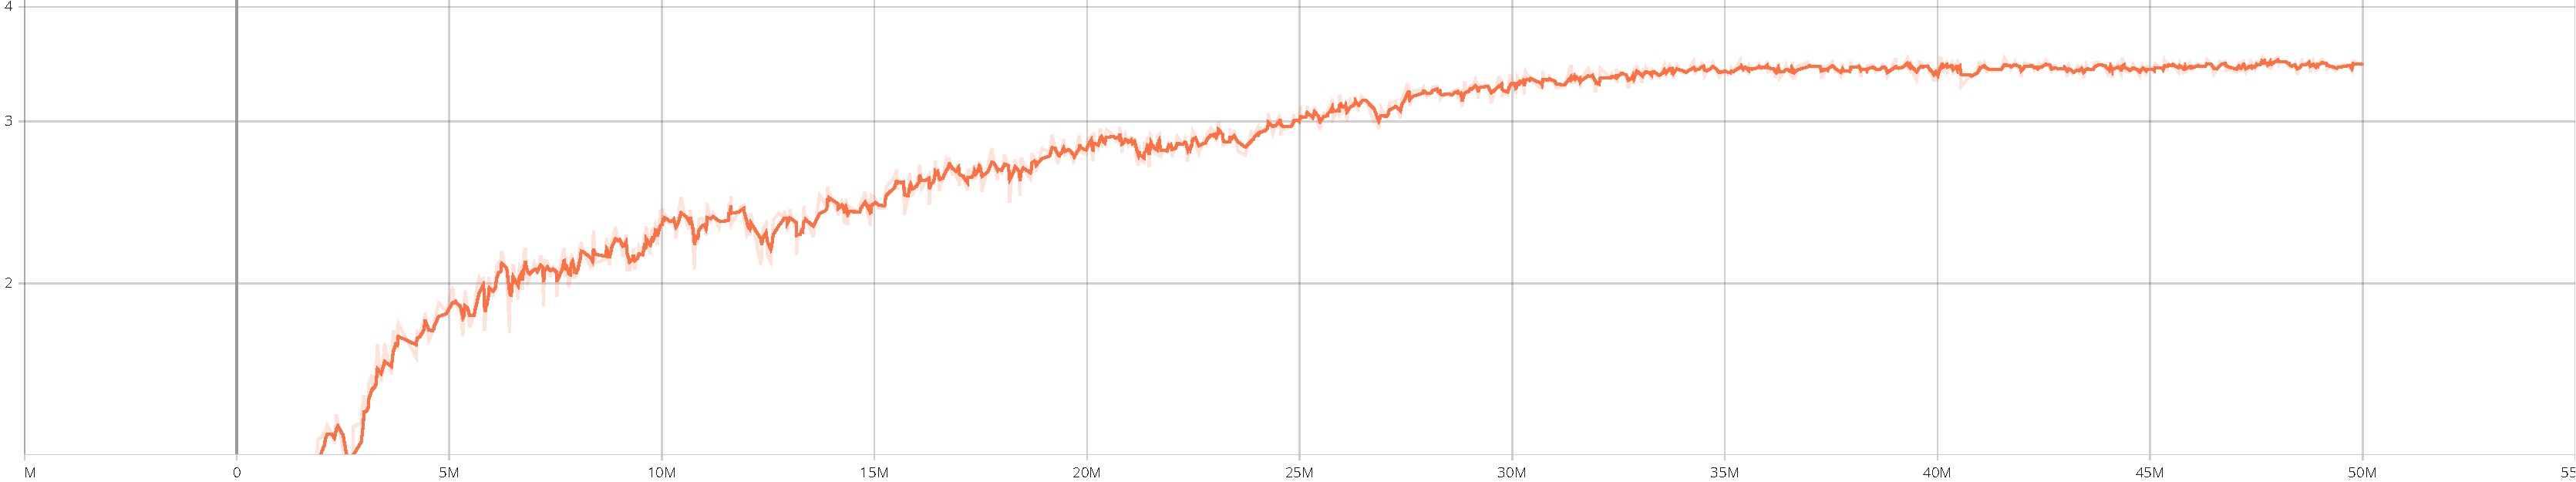
\includegraphics[width=\textwidth]{Bilder/ml-agents/Environment_Cumulative Reward_time-scale-1.pdf}
    \caption{Cumulative Reward der Rekonstruktion von \cite{waidner.2020}}
    \label{fig:time-scale-1}
\end{figure}

Der Verlauf des Cumulative Rewards, der nun beim Training entsteht und in \autoref{fig:time-scale-1} dargestellt wird, gleicht im Wesentlichen den Resultaten von \cite[50]{waidner.2020}.
Auch der gelernte Bewegungsablauf, der bei der Inferenz zu beobachten ist\todo{Video timeScale1}, gleicht den Resultaten der vorangegangenen Arbeit, weshalb die Rekonstruktion als erfolgreich bewertet wird.


\section{Stabilisierung des Laufverhaltens}
Wie in \autoref{sec:probleme} ausgeführt und von den Ergebnissen der Rekonstruktion zusätzlich veranschaulicht wird, bewegt sich der Roboter aktuell mit einer sprungartigen Bewegung fort.
Diese ist, wie beschrieben, Ursache für viele potenzielle Probleme.
Deshalb soll nun das Laufverhalten stabilisiert werden.
In diesem Zusammenhang wird darunter verstanden, die Schwankungen, die die Körpermitte bei der Bewegung vollführt, auf ein Minimum zu begrenzen.
Wird das Vorbild der Spinnen betrachtet, so ist davon auszugehen, dass diese Einschränkung kein Hindernis für eine effiziente Fortbewegung darstellt.

Es existieren innerhalb der Simulation zwei elementare C\#-Skripte, die für die in diesem Kapitel beschriebenen Änderungen von besonderer Relevanz sind: \code{SpiderAgent.cs} und \code{SpiderController.cs}.
In \code{SpiderAgent.cs} befinden sich die für den Reinforcement Learning Prozess relevanten Konfigurationen des Agenten.
Dort werden Beobachtungen gesammelt und dem Lernalgorithmus zur Verfügung gestellt, die Aktionen vom Lernalgorithmus entgegengenommen, die Lern-Episoden verwaltet und vor allem der Reward zugewiesen.
Der \code{SpiderController} ist wiederum einem \code{SpiderAgent} zugeordnet und verwaltet dessen Skripte für die Servomotoren, koordiniert die allgemeine Durchführung der Bewegung und führt das Zurücksetzen der Komponenten durch.
Da ein \code{SpiderController} somit auf die direkten Werte des Roboterzustands zugreifen kann, wird hier auch der Reward berechnet, der in \code{SpiderAgent.cs} zugewiesen wird.

Für die Stabilisierung der Bewegung bestehen nun zwei verschiedene Ansätze, die ausprobiert und verglichen werden.
Beide werden über Änderungen in \code{SpiderController.cs} realisiert.
Die dort implementierte, allgemeine Bewegungskoordination des Roboters ist eine seiner physikalischen Grundeigenschaften und wird deshalb im Rahmen dieser Arbeit nicht manipuliert.
Auch wird so eine kontinuierliche Basis für die einzelnen Versuche und deren Evaluation geboten.
Jedoch stellt der in dieser Klasse berechnete Reward die zentralste Stellschraube des Reinforcement Learning Problems dar.

\begin{figure}
    \lstinputlisting[
        % language = C,
        firstline = 8,
        % lastline = 41,
        caption = Ürsprüngliche Berechnung des Reward-Signals,
        label = code:reward-post-reconstruct
    ]{Code/post-reconstruct/reward.cs}
\end{figure}

In \autoref{code:reward-post-reconstruct} ist die ursprüngliche Berechnung des Rewards zu sehen, wie sie in \code{SpiderController.cs} implementiert ist.
Dabei wird zunächst der Reward mit 0 initialisiert.
Anschließend wird abgeprüft, ob sich der Roboter um mehr als 90° zur horizontalen Achse gedreht hat und eine negative Belohnung vergeben, falls dies der Fall ist.
Mit dieser Prüfung wird verhindert, dass der Roboter sich überschlägt und dabei seine empfindliche Elektronik beschädigt.
Anschließend wird geprüft, wie weit der Roboter auf der Karte in Vorwärtsrichtung von seinem Ausgangspunkt entfernt ist und die Differenz zum vorherigen Resultat dieser Berechnung gebildet.
Diese Differenz -- sowohl wenn diese positiv ausfällt, als auch, wenn sie negativ ist -- wird dann mit der eventuellen Strafe für ein Überschlagen verrechnet und als Reward zurückgegeben.

Der offensichtliche und einfache Weg ist es nun, in der Methode \code{isTurned()} den Schwellwert der Rückgabe von 90° auf einen kleineren Wert, zum Beispiel 5°, zu reduzieren.
Mit dieser Modifikation wird automatisch ein negativer Summand in den Reward eingebracht, wenn die Schwankung der Körpermitte den nun deutlich geringeren Schwellwert überschreitet.
Das Problem hierbei besteht darin, dass die Methode \code{isTurned()} nicht nur zur Berechnung des Rewards verwendet wird, sondern auch in \code{SpiderAgent.cs} die aktuelle Episode terminiert wird, wenn sich der Roboter auf den Rücken dreht.
Wird die beschriebene Modifikation an dieser Methode vorgenommen, so wird auch eine kleine Schwankung der Körpermitte bereits als Überschlag interpretiert und die laufende Trainings-Episode fälschlicherweise beendet.
Wie sich bei einem Trainingsversuch zeigt, führt dies dazu, dass der Roboter kein Laufverhalten lernen kann, da ihm keine Gelegenheit geboten wird, seinen Fehler zu erkennen, zu erforschen und zu korrigieren.
Für eine möglichst stabile Körpermitte sollte der Rotations-Schwellwert möglichst gering sein.
Jedoch wird bei diesem Ansatz ein Training gegenläufig zum sinkenden Schwellwert praktisch unmöglich.

\begin{figure}
    \lstinputlisting[
        % language = C,
        % firstline = 8,
        lastline = 18,
        caption = Reward-Funktion mit Stabilisierung,
        label = code:reward-1-adjustAngle
    ]{Code/1-adjustAngle/reward.cs}
\end{figure}

Eine alternative Lösung ist in \autoref{code:reward-1-adjustAngle} dargestellt.
Zentrales Element dieser Lösung ist die neu eingeführte Methode \code{getAngle()}.
Der Methodenrumpf ist fast identisch mit dem der Methode \code{isTurned()} aus \autoref{code:reward-post-reconstruct}.
Der Unterschied besteht dabei darin, dass die neue Methode nicht prüft, ob der berechnete Winkel größer als 90° ist und den resultierenden Wahrheitswert zurückgibt, sondern stattdessen den Rest der Division des Winkels durch 90 bestimmt und als Fließkommazahl zurückliefert.
Anschließend wird der mit der neuen Methode berechnete Winkel mit einem kleinen negativen Faktor multipliziert und dieser Summand in der Berechnung des Rewards ergänzt (Zeile 6).
Somit wird eine Strafe vergeben, deren Betrag proportional mit der Rotation der Körpermitte zunimmt.
Die anschließende Belohnung für die zurückgelegte Distanz und die Verrechnung mit der Bestrafung bleibt unverändert.

\begin{figure}
    \centering
    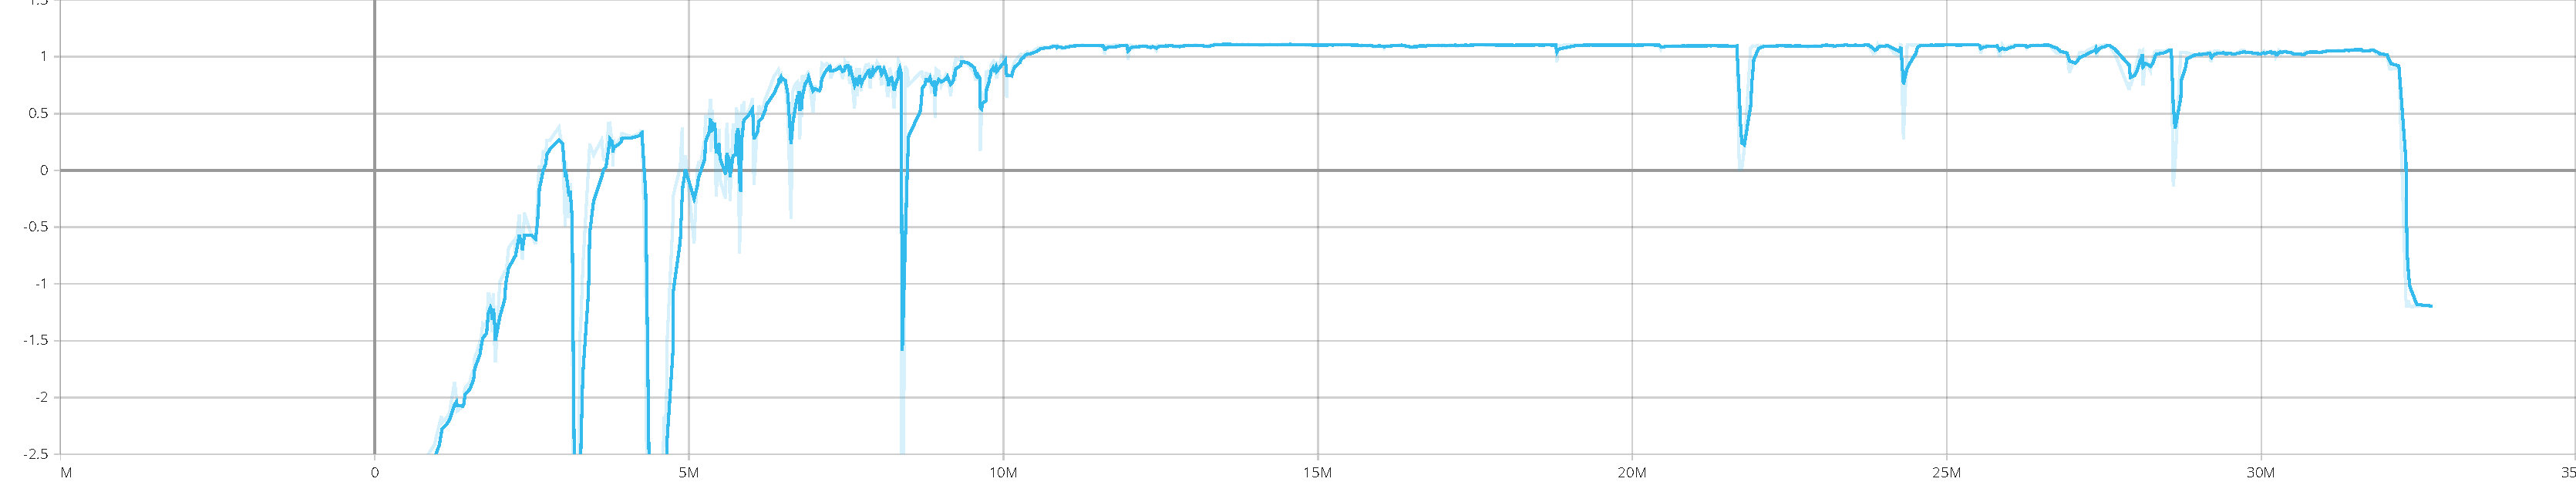
\includegraphics[width=\textwidth]{Bilder/ml-agents/Environment_Cumulative Reward_adjustedAngles.pdf}
    \caption{Cumulative Reward mit Stabilisierung}
    \label{fig:adjustedAngles}
\end{figure}

Das mit dieser Reward-Funktion trainierte Modell legt die Wirksamkeit der Maßnahme dar: beim Laufverhalten des Roboters ist zu beobachten, dass die Körpermitte perfekt in einer horizontalen Lage gehalten wird.
\autoref{fig:adjustedAngles} zeigt den Verlauf des Cumulative Rewards während des Trainings.
Im Vergleich zu \autoref{fig:time-scale-1} fällt auf, dass der Trainingsprozess zwar zu einem stabilen Wert konvergiert, jedoch besonders am Anfang deutlich instabiler verläuft.
Außerdem ist der Wert, zu dem das Training konvergiert, fast um zwei Drittel gemindert.
Betrachtet man das Laufverhalten des Roboters\todo{Video adjustedAngles}, so fällt weiterhin auf, dass der Roboter weiterhin eine sprungartige Fortbewegung wählt.
(Diese fällt allerdings weitaus stabiler aus, als der in \cite{waidner.2020} erlernte Bewegungsablauf.)
Dabei werden allerdings nur die beiden vorderen und eins der hinteren Beine verwendet, das letzte Bein ist eingekringelt und berührt den Boden nicht.

\subsection{Optimierung der Reward-Funktion}
In einem Versuch, das Laufverhalten weiter zu optimieren und eine natürlichere Laufbewegung zu erhalten, wird die Berechnung des Rewards leicht umgestaltet.
Die optimierte Version ist in \autoref{code:reward-4-no-box} abgebildet.
Die Prüfung, ob der Roboter sich überschlagen hat, bleibt bestehen, wobei hier die Bestrafung erhöht wird, um den Überschlag als schlimmstmöglichen Fall vom instabilen Laufverhalten abzugrenzen.
Tritt dieser Fall ein, so findet auch keine weitere Berechnung des Rewards statt, sondern der Wert der Strafe wird umgehend zurückgegeben.
Danach wird eine kleine Strafe eingeführt, die mit jedem Schritt vergeben wird.
Diese stellt eine generelle Optimierung der Reward-Funktion dar, da eine solche Strafe bewirkt, dass ein Agent danach strebt, sein Ziel möglichst schnell zu erreichen \cite{mlagentsReward}.

Durch die starke Modifikation der Gewichte in der Reward-Funktion können die Beträge der Cumulative Reward Funktion während des Trainings nicht mehr als vergleichende Metrik eingesetzt werden.
Der in \autoref{fig:4-debug} dargestellte Kurvenverlauf zeigt jedoch, dass der Trainingsprozess bedeutend stabiler verläuft verglichen mit \autoref{fig:adjustedAngles}.
Das in Folge der vorgenommenen Maßnahmen trainierte Modell zeigt ein erstaunlich natürliches Bewegungsmuster, sehr ähnlich zur Fortbewegung eines Spinnentiers.
\todo{Video 4-debug-extended-vector-size}

\begin{figure}
    \lstinputlisting[
        % language = C,
        % firstline = 8,
        lastline = 12,
        caption = Optimierte Reward-Funktion,
        label = code:reward-4-no-box
    ]{Code/4-no-box/reward.cs}
\end{figure}


\begin{figure}
    \centering
    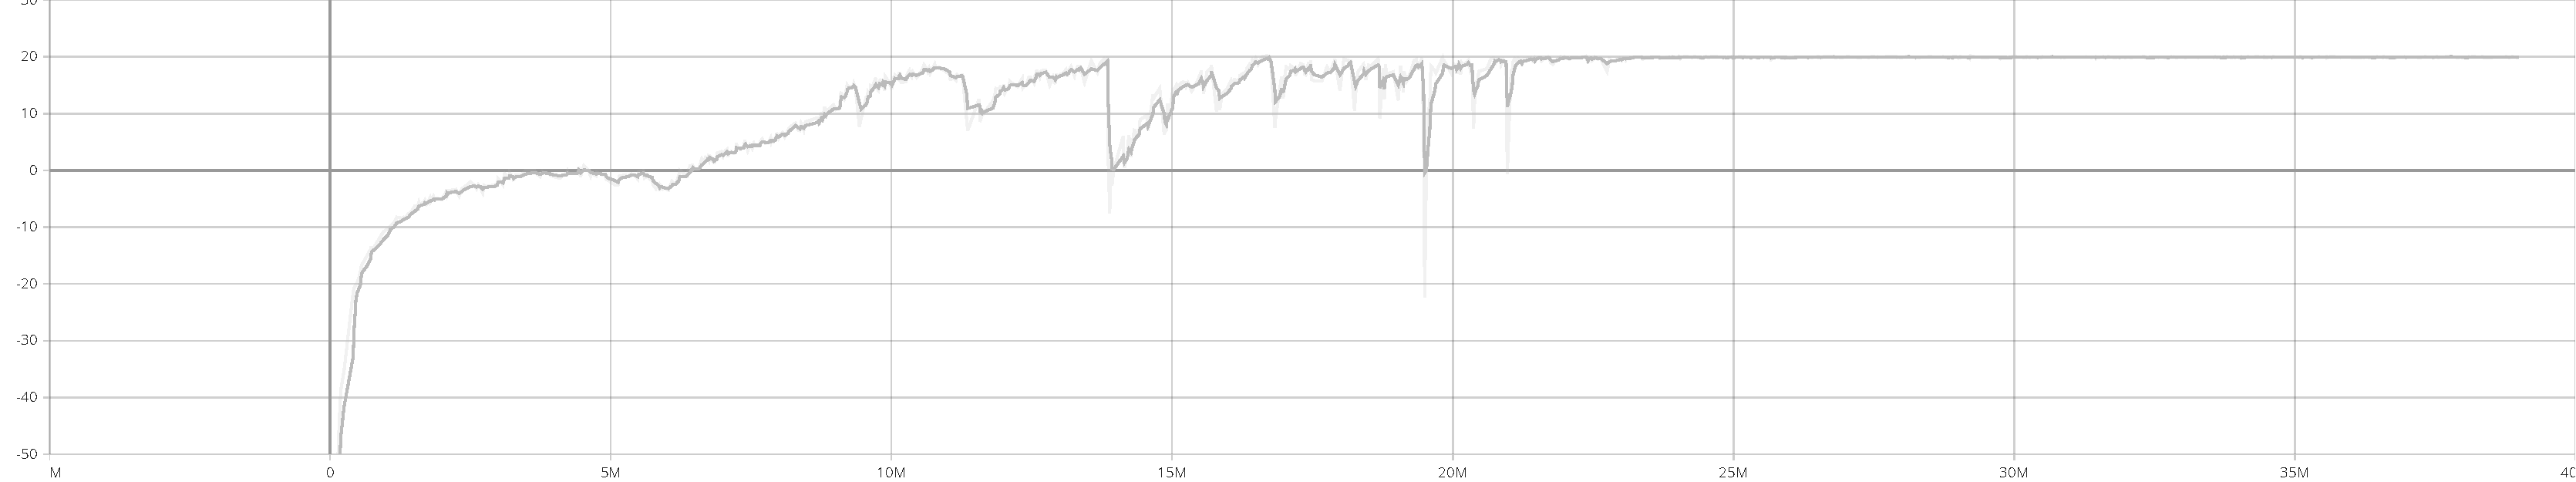
\includegraphics[width=\textwidth]{Bilder/ml-agents/Environment_Cumulative Reward-4-debug-extended-vector-space.pdf}
    \caption{Cumulative Reward mit Optimierung der Reward-Funktion}
    \label{fig:4-debug}
\end{figure}


\section{Pfadplanung}
Der nächste Implementierungsschritt ist die Ergänzung von Pfadplanung.
Hierfür wird zunächst ein Proof of Concept erstellt und dieses im Anschluss auf den Roboter übertragen.

\subsection{Proof of Concept: Crawler}
Wie in \autoref{sec:realisierung} erwähnt, bietet das \emph{Crawler-Example} des ML-Agents-Toolkits eine interessante Referenz für die Pfadplanung.
Im Beispiel wurde ein Agent darauf trainiert, nacheinander zu zufällig erscheinenden Zielen zu laufen.
Wenn der Agent ein Ziel (\emph{DynamicTarget}) erreicht, so verschwindet es und taucht an anderer Stelle wieder auf.
Der Agent hat dabei keinen Einfluss auf das DynamicTarget und kennt nur dessen aktuelle Position.

Wenn ein DynamicTarget initialisiert wird oder in Kontakt mit einem Unity-GameObject kommt, welches mit dem Tag \enquote{agent} versehen ist, wird die in \autoref{code:dynamic-target-old} dargestellte Methode ausgeführt, welche das DynamicTarget an einen zufälligen Ort teleportiert.

\begin{figure}
    \lstinputlisting[
        % language = C,
        % firstline = 8,
        % lastline = 12,
        caption = Respawnen des DynamicTargets,
        label = code:dynamic-target-old
    ]{Code/crawler/TargetController-extract.cs}
\end{figure}

Mittels der Modifikation aus \autoref{code:dynamic-target-new} ist es möglich, Einfluss auf die Reihenfolge zu nehmen, in der die DynamicTargets erscheinen.
Die Kontrollstruktur basiert auf einem Zähler und einer Liste von Positionen (Zeile 1f).
Solange der Zähler mit einem Listenindex korrespondiert (Zeile 5), wird als neue Position des Ziels die in der Liste hinterlegte Position verwendet.
Wurde die Liste vollständig abgearbeitet, erscheinen die Ziele wieder zufällig.
In der Element-Detailansicht von Unity können anschließend beliebig viele Zielpunkte frei eingegeben werden (\autoref{fig:eingabefeld-positionen}).

\begin{figure}
    \lstinputlisting[
        % language = C,
        % firstline = 8,
        % lastline = 12,
        caption = Modifiziertes Respawnen des DynamicTargets,
        label = code:dynamic-target-new
    ]{Code/crawler/PathTargetController-extract.cs}
\end{figure}

\begin{figure}
    \centering
    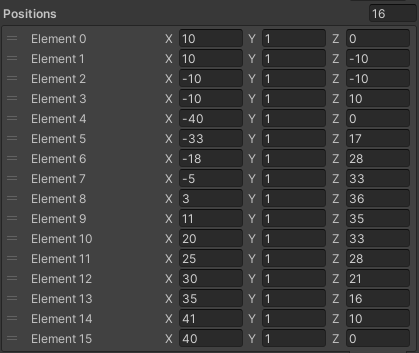
\includegraphics[width = 0.5\textwidth]{Bilder/crawler/position-list.png}
    \caption{Eingabefeld der Positionen}
    \label{fig:eingabefeld-positionen}
\end{figure}

Da der Agent im Crawler-Example die Ziele nicht selbst kontrolliert, ist kein erneutes Trainieren des Modells nötig, sondern die Modifikationen sind direkt wirksam und der Agent läuft entlang des vorgegebenen Pfades.\todo{Video crawler-poc}

\subsection{Übertragung auf den SpiderAgent}
Um dieses Prinzip für den Roboter in dieser Studienarbeit zu nutzen, werden der \code{TargetController} und das dazugehörige Prefab aus dem Beispielprojekt des ML-Agents-Toolkits in die Simulationsumgebung kopiert.
\code{SpiderAgent.cs} wird im Anschluss um den in \autoref{code:dynamic-target-spawn} dargestellten Code ergänzt.
Dieser stellt eine Verknüpfung zwischen dem Agent und dem Target her und ermöglicht das initiale Spawnen des Ziels.
Weiterhin wird sämtlichen Körperteilen des Roboters der Tag \enquote{agent} zugewiesen.
Für das Training wird die Positionsliste leer gelassen, um die Targets zufällig auf der Trainingsplattform erscheinen zu lassen, damit der Roboter nicht einen vorgegebenen Pfad auswendig lernt.


\begin{figure}
    \lstinputlisting[
        % language = C,
        % firstline = 8,
        % lastline = 12,
        caption = Ergänzung für Spawnen des Targets (SpiderAgent.cs),
        label = code:dynamic-target-spawn
    ]{Code/targetAddition.cs}
\end{figure}

Bislang verfügt der Roboter nur über die aktuellen Winkel der Servomotoren als Observations.
Für das weitere Training sollen ihm nun zusätzlich seine eigene Position und die Position des Ziels zugänglich gemacht werden, da es für den Algorithmus andernfalls nicht möglich ist, seine Aktionen auf das Erreichen des Ziels auszurichten.
Alternativ könnte dem Roboter ein Richtungsvektor übergeben werden, der vom Roboter auf das Ziel zeigt.
Hinsichtlich ihres Informationsgehalts sind beide Angaben identisch, da sie rechnerisch ineinander überführt werden können.
Da bei der manuellen Berechnung des Richtungsvektors jedoch leichter Fehler auftreten können, werden absolute Positionen übergeben.
Außerdem wird dadurch zukünftig das Verbinden eines beliebigen Ortungssystems potenziell einfacher gehalten.

Als Voraussetzung, um die zusätzlichen Informationen zur Verfügung zu stellen, muss in Unity die Größe des Observation Space um sechs Elemente erhöht werden, da beide zu übergebenden Positionen jeweils von einem dreidimensionalen Vektor repräsentiert werden.
Anschließend wird die in \autoref{code:observations} dargestellte Methode zum Sammeln der Observations modifiziert.
Vor der Modifikation bestand die Methode lediglich aus der Schleife, die die einzelnen Werte der Servomotoren ausliest und in den VectorSensor eingibt.
Diese Informationen werden um die beiden zusätzlichen Positionen ergänzt.
Die gesamte Anzahl aller Einträge, die in dieser Methode zugewiesen werden muss exakt der in Unity hinterlegten Größe des Observation Space entsprechen, ansonsten erzeugt die Methode Fehler.

\begin{figure}
    \lstinputlisting[
        % language = C,
        % firstline = 8,
        % lastline = 12,
        caption = Erweiterung des Observation Space (SpiderAgent.cs),
        label = code:observations
    ]{Code/extendedVectorSpace/observations.cs}
\end{figure}

\subsection{Geometrische Reward-Funktion}
Um den Roboter nun dazu zu animieren, nicht mehr geradeaus, sondern zu den Zielen zu laufen, wird die Reward-Funktion angepasst.
Wie in \autoref{sec:realisierung} beschrieben, existieren dafür verschiedene Ansätze.
Als der vielversprechendste erscheint dabei die Verwendung einer sogenannten geometrischen Funktion.
Kennzeichnend für diese ist, dass die einzelnen Bestandteile des Rewards nicht wie bislang aufsummiert werden, sondern ein Produkt aller Faktoren gebildet wird.
Damit soll vermieden werden, dass sich der Agent darauf konzentriert, den einfachsten Reward zu maximieren und damit etwa in einem lokalen Maximum stecken zu bleiben.
Um das Produkt zu maximieren, müssen zwangsläufig alle einzelnen Faktoren maximiert werden.

Es werden Trainings für drei solcher Funktionen durchgeführt.
Die Funktionen haben verschiedene Komplexitäten und Ansätze, um eine allgemeine Eignung einer solchen Reward-Funktion abzuschätzen.
\begin{itemize}
    \item Für den ersten Ansatz wird die Distanz gemessen, die der Roboter seit dem letzten Schritt zurückgelegt hat.
    Ausschlaggebend für die Messung ist dabei nur die Körpermitte.
    Als zusätzlicher Faktor wird der Winkel zwischen der \enquote{Blickrichtung} der Körpermitte und der relativen Richtung, in der das Ziel liegt, gebildet und auf einen Bereich von 180° normalisiert.

    \item Die zweite Variation verwendet die in Unity-GameObjects hinterlegte Geschwindigkeit der einzelnen Körperteile und bildet daraus den Durchschnitt.
    Dieses Vorgehen soll plötzliche und ruckartige Bewegungen des Roboters, die beim Training auftreten, ausgleichen.
    Der nächste Faktor ist, wie bei der ersten Variante, ein normalisierter Wert an dem abgelesen werden kann, ob die Bewegung in Richtung Ziel erfolgte.
    Weiterhin wird hier wieder eine Belohnung eingeführt, die umso höher ausfällt, desto stabiler die Körpermitte in der Horizontalen gehalten wird.

    \item Der letzte Ansatz ist sehr ähnlich zum zweiten.
    Allerdings wird hier auf das berechnete Produkt noch eine konstante Strafe für jeden Schritt summiert, um eine schnelle Zielerreichung voranzutreiben.
\end{itemize}

Trotz der Unterschiede der Ansätze zeigen alle ein ähnliches Ergebnis des Trainings: der Roboter fällt mit seiner Körpermitte auf den Boden und bewegt seine Beine in der Luft.
Der Cumulative Reward ist dabei relativ konstant, das Modell lernt auch nach mehreren Millionen Simulationsschritten nicht.

\subsection{Klassischer Reward}
\label{sec:classic-reward}
Aus diesen Gründen wird die Entscheidung getroffen, die Reward-Funktion neu zu entwerfen und dabei möglichst wenig konzeptionelle Änderungen ausgehend vom stabilisierten Laufverhalten vorzunehmen.
Ziel dieser Vorgehensweise ist es, die Quellen potenzieller Fehler möglichst weit einzuschränken.
Es wird grundlegend dieselbe optimierte Reward-Funktion wie in \autoref{code:reward-4-no-box} genutzt.
Der Unterschied besteht hierbei jedoch darin, dass nicht mehr die zurückgelegte Distanz entlang der x-Achse gemessen wird, sondern die zurückgelegte Distanz in Richtung des Ziels.
Dafür wird die jeweils letzte Position des Roboters zwischengespeichert.
Es werden dann die Distanzen von der letzten Position zur Zielposition sowie von der aktuellen Position zur Zielposition gebildet.
Anschließend wird die Differenz der beiden Distanzen so bestimmt, dass die Berechnung in einer positiven Belohnung resultiert, wenn der Roboter sich dem Ziel genähert hat.

Dieser Ansatz zeigt bessere Ergebnisse als die mit geometrischer Reward-Funktion, jedoch wird im Training sehr früh ein lokales Maximum erreicht.
Dabei lernt der Roboter, dass er eine Belohnung erzielt, wenn er sich in Richtung des Ziels rollen lässt, überschlägt sich dabei allerdings und startet somit die Trainingsepisode neu.
Versuche, die Strafen für Überschlagen und Körperrotation anzuheben, schlagen ebenfalls fehl.
Wird diese Maßnahme ergriffen, verschlechtern sich die Resultate sogar.
Anstatt sich in Richtung des Ziels zu rollen, rollt sich der Roboter auf dem Boden ein und vollführt nur minimale Bewegungen.

\subsection{Optimierung der Hyperparameter}
Aufgrund der geringen Abweichung der aktuellen Reward-Funktion von \autoref{code:reward-4-no-box} und des simplen Aufbaus der Funktion wird ein Logikfehler in der Funktion als Ursache ausgeschlossen.
Zur Fehlersuche werden erneut Testreihen ausgehend vom Stand des stabilisierten Laufverhaltens durchgeführt und dabei die Änderungsschritte zusätzlich verkleinert.
Dieser letzte Stand enthält als Observationen nur die Winkel der zwölf Servomotoren.
Im ersten Schritt wird nun die Größe des Observation Space erneut, wie oben beschrieben, erweitert.
Dabei werden allerdings nicht die Position des Roboters und die des Ziels hinzugefügt, sondern zwei dreidimensionale Nullvektoren als Platzhalter.
Wie erwartet ist der Cumulative Reward des Trainingsdurchlaufs praktisch deckungsgleich mit dem Stand vor der Veränderung.
Der nächste Schritt fügt nun bei weiterhin gleichbleibender Reward-Funktion die beiden Positionen als Beobachtung anstelle der Nullvektoren hinzu.
Auch wenn zusätzliche Informationen, die allerdings nicht in den Reward einfließen, den Trainingsprozess eigentlich nicht negativ beeinflussen dürften, erreicht der Trainingsprozess mit Zugriff auf die Positionen keinen positiven Cumulative Reward.

Die wahrscheinlichste Ursache für ein solches Verhalten sind suboptimal eingestellte Hyperparameter.
Zusätzlich scheint die Anzahl der Neuronen des verwendeten Neuralen Netzes für die gesteigerte Eingabekomplexität nicht mehr auszureichen.
Aufgrund der Ähnlichkeit des Problems mit dem Crawler-Example, werden die Hyperparameter beider Probleme miteinander abgeglichen und optimiert zusammengeführt.
\autoref{fig:optimierte-hyperparameter} zeigt eine Übersicht der Cumulative Rewards der drei Testläufe.
Die optimierten Hyperparameter werden in \autoref{anhang:trainer-config} dargestellt.

\begin{figure}
    \centering
    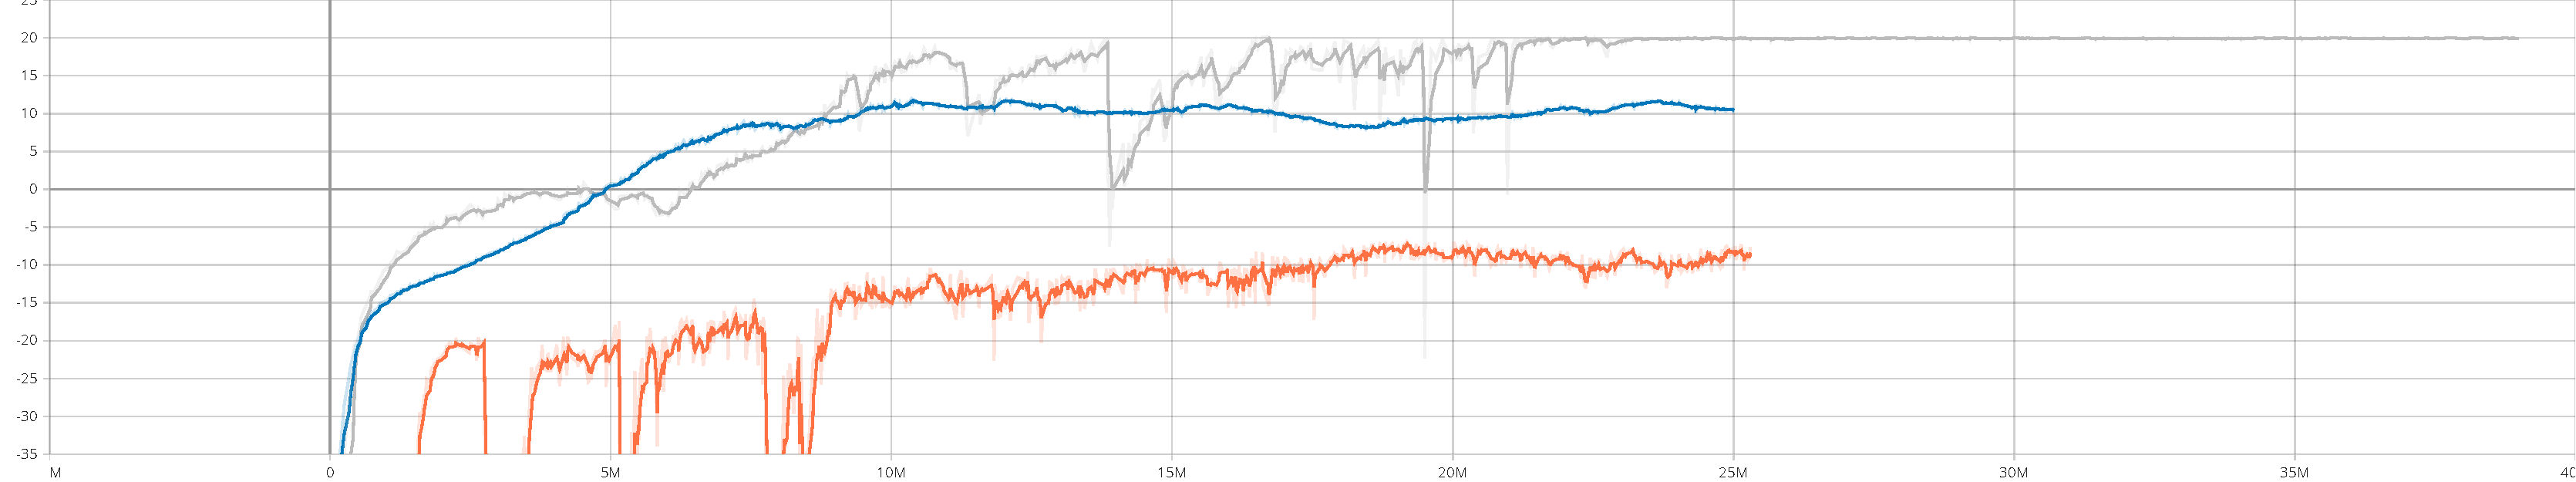
\includegraphics[width = \textwidth]{Bilder/ml-agents/Environment_Cumulative Reward-add-observations.pdf}
    \caption[Schrittweise Erweiterung und Optimierung der Hyperparameter]{Schrittweise Erweiterung und Optimierung der Hyperparameter: (grau) hinzugefügte Nullvektoren; (orange) zusätzliche Beobachtungen bereitgestellt; (blau) optimierte Hyperparameter}
    \label{fig:optimierte-hyperparameter}
\end{figure}

Auf Basis der neu eingestellten Hyperparameter werden erneut die Änderungen von \autoref{sec:classic-reward} angewandt.
Als Resultat kann zwar eine stabil ansteigende Kennkurve des Cumulative Reward beobachtet werden, jedoch trifft dies nicht auf das gelernte Bewegungsverhalten zu.
Der Roboter vollführt eine Mischung aus Sprüngen und Schritten, die ihn teilweise zielstrebig auf das Ziel zubewegen, in anderen Situationen jedoch vollkommen zufällig erscheinen.\todo{video 14a}
In der Dokumentation von ML-Agents wird als Maßnahme für einen stabilen Trainingsprozess empfohlen, den Betrag des Rewards möglichst auf einen Betrag von 1 zu skalieren.
Einige Versuche mit verschiedenen Skalierungen zeigen jedoch keine abweichenden Ergebnisse.
Auffällig ist jedoch, dass die Cumulative Rewards der Trainingsdurchläufe mit skalierten Rewards deutlich stärker schwanken (\autoref{fig:scale-reward}).

\begin{figure}
    \centering
    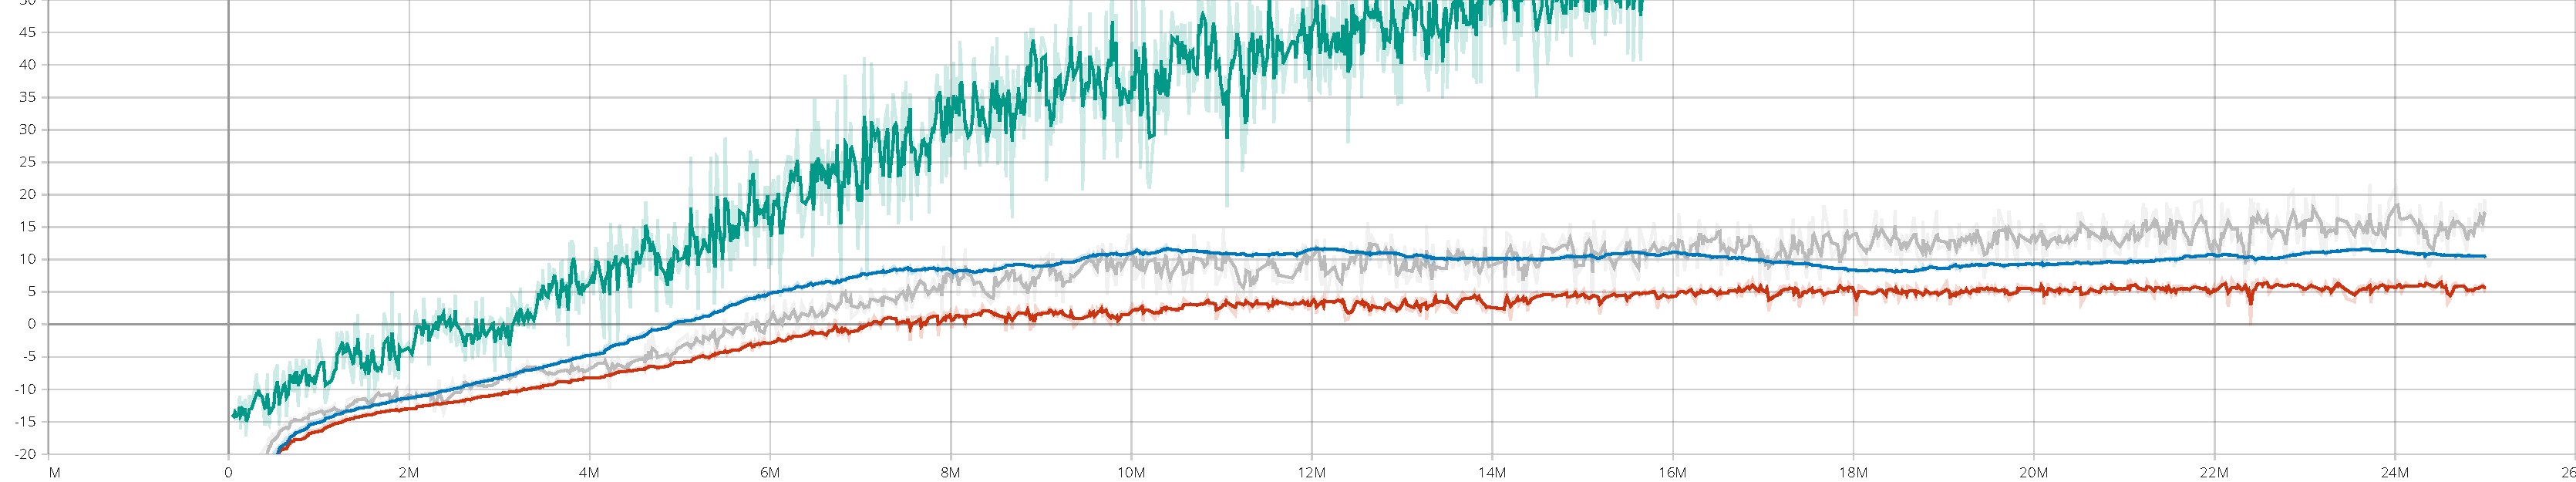
\includegraphics[width = \textwidth]{Bilder/ml-agents/Environment_Cumulative Reward-scale-reward.pdf}
    \caption[Vergleich verschiedener Skalierungen des Rewards]{Vergleich verschiedener Skalierungen des Rewards: (blau) Vergleichskurve geradeaus laufen; (rot) Belohnung für Bewegung in Richtung des Ziels; (grün) skalierter Reward; (grau) skalierter Reward mit höheren Strafen für Schieflage der Körpermitte}
    \label{fig:scale-reward}
\end{figure}

\section{Hindernisumfahrung}
Da Hindernisse nur im Kontext eines vorgesehenen Pfades sinnvoll umsteuert werden können, ist eine funktionierende Pfadplanung eine notwendige Voraussetzung für ein erfolgreiches Training eines Modells, dass den Roboter Hindernisse umsteuern lässt.
Da die im vorherigen Kapitel trainierte Pfadverfolgung keine verwendbare Basis darstellt, werden im Folgenden ein paar grundlegende Aspekte thematisiert und demonstriert.

Um zu sehen, wie der Roboter auf einem einfachen Pfad auf ein statisches Hindernis reagiert, werden ein paar Experimente auf Basis des laufstabilisierten Modells durchgeführt.
Als Pfad ist hier das Laufen entlang der x-Achse zu betrachten, wobei anzumerken ist, dass es keinen Faktor gibt, der eine seitliche Abweichung entlang der z-Achse korrigieren würde.
Stellt man dem normal trainierten Modell ein Hindernis orthogonal zu seiner Laufrichtung in den Weg, so kann man beobachten, dass der Roboter bis an das Hindernis läuft und auch nach der Kollision seine Gangbewegung noch unverändert ausführt, dabei seine Beine allerdings nur auf der Stelle über den Boden schiebt.
Von solch einem Ergebnis ist ohne explizites Training auch auszugehen, da der Roboter nie lernt, zur Seite zu gehen.

Wird nun allerdings mit unveränderter Reward-Funktion und zusätzlich mit dem eingefügten Hindernis trainiert, kann ein interessantes Ergebnis beobachtet werden.
Wie in \autoref{sec:realisierung} schon ausgeführt, lernt der Roboter seine Umgebung auswendig, wenn sich diese nicht verändert.
Dies ist auch hierbei zu beobachten.
Was allerdings verwundert, ist, dass der Roboter schon zu Beginn anfängt, eine Kurve zu laufen, mit der er knapp am Hindernis vorbeikommt -- jedoch wird diese Kurve nicht abgebrochen, wenn der Roboter am Hindernis vorbeilaufen kann, obwohl er dadurch ausschließlich negative Rewards bekommen kann.
Dies widerspricht eigentlich einer der grundlegendsten Maxime von Reinforcement Learning: den Reward immer und um jeden Preis zu maximieren.

Im Falle des Crawler-Examples, anhand dessen ein Proof of Concept zur Pfadplanung implementiert wurde, kann ähnliches beobachtet werden wie bei dem Modell des SpiderAgents, welches nicht explizit für das Hindernis trainiert wurde.
Aufgrund seiner physikalischen Simulationseigenschaften federt der Crawler etwas von der Wand zurück, gegen die er wiederholt läuft.
Dabei wird er jedes Mal leicht zur Seite abgedrängt, wodurch er nach einiger Zeit das Hindernis überwindet.
Dieser Vorgang ist jedoch weder eine gezielte Handlung noch ansatzweise effizient.\todo{Video crawler wand}

Diese Experimente zeigen anschaulich, dass auch bei bereits funktionierender Pfadplanung in jedem Fall ein gesondertes Training mit einem zufällig generierten Hindernisparcour notwendig ist, um dem fertigen Modell ein Umsteuern von Hindernissen zu ermöglichen.
Für den Fall, dass das Erlernen von Pfadplanung und das gleichzeitige Umsteuern von Hindernissen ein zu komplexes Lernproblem darstellt, könnte gegebenenfalls Curriculum Learning eingesetzt werden, um die Probleme aufeinander aufbauend zu lösen.
Insgesamt dürfte eine Hindernisumsteuerung langfristig nur sinnvoll sein, wenn sie mit Sensorik unterstützt wird.
Da dies das Problem und dessen Komplexität deutlich verändert, wird dann allerdings ohnehin ein gesondertes Training notwendig sein.
\chapter{Bewertung der Ergebnisse}
\begin{itemize}
    \item Unterschiede zu Crawler-Example
    \item denkbar sind Fehler in der Simulation der Servomotoren, die zu einem unrealistischen Ergebnis führen
    \item evaluieren, um welche Sensoren der Roboter in der Realität sinnvoll ergänzt werden könnte und dem Roboter mehr Informationen über sich selbst bereitstellen; Mangel an Informationen wurde hier als Grunddefinition gesetzt, ist jedoch elementarster Unterschied zu vergleichbaren Projekten, welche allerdings deutlich erfolgreichere Ergebnisse vorweisen
    \item herausfinden, warum Policy Loss / Value Loss so hoch sind und wie das Training nachhaltig stabilisiert werden könnte
\end{itemize}
\chapter{Fazit}
Ziel dieser Arbeit war es, ein vorliegendes Reinforcement Learning Problem, bei dem einem spinnenartiger Roboter das Laufen beigebracht wird, um Pfadplanung und das Umsteuern von Hindernissen zu erweitern.
Dazu wurden zunächst wichtige Grundlagen erläutert und der State of the Art von Reinforcement Learning gesteuerter Lokomotion vorgestellt.
Anschließend wurde ein Konzept zur Lösung der Aufgabe erarbeitet.
Dabei wurden vor allem notwendige Modifikationen am Roboter und Möglichkeiten zur Pfadplanung diskutiert.
Die gewählte Realisierung soll dem Roboter generische Positionierungsinformationen bereitstellen.
Weiterhin wird ein Pfad nicht als ganzes betrachtet, sondern in einzelne Punkte zerlegt.
Das Erreichen des jeweils nächsten Punktes kann auf das Ausgangsproblem reduziert werden.

Gemäß dem entwickelten Konzept wurde die Trainingsumgebung an den aktuellen Stand der Technik angepasst und verschiedene Testreihen mit dem \acl{ppo}-Algorithmus durchgeführt.
Dabei wurde erfolgreich das zuvor Sprung-basierte Laufverhalten des Roboters stabilisiert.
Für die Pfadplanung wurde, anhand eines ähnlich aufgebauten Projekts, erfolgreich ein Proof of Concept implementiert.
Das Training am eigenen Roboter war nur eingeschränkt erfolgreich, wobei als primäre Fehlerquellen die Hyperparameter des Trainings und ein Mangel an zur Verfügung gestellten Informationen vermutet werden.
Die Trainingsdurchläufe wurden anhand geeigneter Metriken analysiert und Vorschläge für zukünftige Verbesserungen dargelegt.
Ein sinnvolles Training der Hindernisumfahrung konnte nicht durchgeführt werden, da dieses auf der Verfolgung eines vorgegebenen Pfads aufbaut.
Trotz dieser Schwierigkeiten wurden mehrere Tests durchgeführt, um die Möglichkeiten der Hindernisumfahrung zu evaluieren und die weitere Roadmap zu beschreiben, wenn eine funktionierende Pfadplanung als Basis erreicht wurde.

% ---- Literaturverzeichnis
\cleardoublepage
\renewcommand*{\chapterpagestyle}{plain}
\pagestyle{plain}
\pagenumbering{Roman}                   % Römische Seitenzahlen
\setcounter{page}{\numexpr\value{savepage}+1}
\printbibliography[title=Literaturverzeichnis]

% ---- Anhang
\appendix
\chapter{Hinweis}
Der vollständige Quellcode sämtlicher Trainingsschritte ist frei verfügbar unter \url{https://github.com/MobMonRob/HindernisumfahrungRLStudien} sowie unter \url{https://github.com/yschiebelhut/spider_bot_rl_training}.
Weiterhin enthält \url{https://github.com/yschiebelhut/spiderbot-training-data} die für Linux kompilierten Trainingsumgebungen, die trainierten Modelle und alle notwendigen Daten, um die Trainingsprozesse mit Tensorboard nachvollziehen zu können.

\paragraph{Wichtig:} Zur Durchführung der Inferenz eines bestimmten Modells sollte das Haupt-Repository möglichst auf dem entsprechenden Commit ausgecheckt sein, auf dem das Training stattgefunden hat.
(Die Numerierungen in den Commits und den Run-IDs geben darüber Aufschluss.)
Dies ist wichtig, da insbesondere die Größe des Observation Space als auch die Observations selbst mit den beim Training verwendeten Daten übereinstimmen müssen, weil es ansonsten zu Fehlern bei der Interpretation des neuronalen Netzes kommt.


\chapter{ML-Agents Training Konfiguration}
\label{anhang:trainer-config}
\begin{figure}[H]
    \lstinputlisting[
        label = code:trainer-config-yaml
    ]{Code/new-trainer-config.yaml}
\end{figure}
%\clearpage
%\pagenumbering{Roman}  % römische Seitenzahlen für Anhang

\newpage
\end{document}
